\documentclass[12pt]{article}

% \usepackage[latin1]{inputenc}    
\usepackage[T1]{fontenc}
\usepackage[french]{babel} 
\usepackage[utf8]{inputenc} 
\usepackage{amsmath, amssymb}
\usepackage[top=2.5cm, bottom=2.5cm, left=2cm, right=2cm]{geometry}
\usepackage{graphicx}
\usepackage{float}
\usepackage{titlesec}
\usepackage{gensymb}
\usepackage[bookmarks,hypertexnames=false,debug]{hyperref}
\usepackage{bookmark}
\usepackage[toc,page]{appendix}

\usepackage{xcolor}
\definecolor{backcolour}{rgb}{0.95,0.95,0.92}
\usepackage{minted}
\newmintinline[mypython]{python}{}
\newminted{python}{fontsize=\scriptsize, 
                   linenos,
                   numbersep=8pt,
                   gobble=4,
                   frame=lines,
                   bgcolor=backcolour,
                   framesep=3mm} 
\usepackage{listings}

\usepackage[style=apa]{biblatex}
\addbibresource{src/bibs.bib}

\usepackage{setspace} \onehalfspacing % interline interval

\setlength{\parindent}{1.25cm} 
\setlength{\parskip}{1em}

\usepackage{todonotes} % To write organized to-do notes
\reversemarginpar % To put notes on the left side
\newcommand{\todolink}{\todo[fancyline, size=\scriptsize]{TOCITE}}
\newcommand{\todounderline}[1]{\todo[inline, size=\scriptsize]{#1}}
\newcommand{\todoinline}[2]{\todo[noinlinepar, inline, inlinewidth=#1, size=\scriptsize]{#2}}

% footers and headers
\usepackage{fancyhdr}
\pagestyle{fancy} 
\fancyhead{}
\fancyfoot{}
\fancyfoot[R]{\thepage}
% \fancyhead[L]{École Nationale des Ponts et Chaussées - Projet de fin d'Etudes}
% \fancyfoot[L]{Latyshev Andrey - Département Génie Mécanique et Matériaux}
\fancyhead[L]{École Nationale des Ponts et Chaussées - End-of-studies project}
\fancyfoot[L]{Latyshev Andrey - Department of Mechanical Engineering and Materials}

\renewcommand{\headrulewidth}{0.0pt}

\usepackage{src/Latyshev_style}

\begin{document}

\begin{titlepage}
	{
        \center
	    \includegraphics[width=40mm]{img/ENPC_logo.png}\\[.44cm]
	    {\large École des Ponts ParisTech}\\[0.2cm]
	    {\normalsize 2021-2022}\\[.64cm]

	    {\Large End-of-studies project}\\[.5cm]
        {\large Department of Mechanical Engineering and Materials}\\[.85cm]
        {\Large Andrey Latyshev}\\[1cm]    
        {\large Double degree engineering student}\\[.85cm]

        {\Large Finite-element implementation of standard and softening plasticity using a convex optimization approach}\\[1cm]
        {\normalsize Project carried out within Laboratoire Navier, ENPC}\\[0.2cm]
	    {\normalsize 6 et 8 avenue Blaise Pascal, Champs-sur-Marne, 77455}\\[0.2cm]
        {\normalsize 21/03/2022 - 09/09/2022}\\[1.1cm]

        {\large Tutor: Jeremy Bleyer}\\[1.1cm]
    }
    \noindent \textbf{\normalsize Composition of jury}\\
    {\normalsize President: Dr. Karam Sab}\\
    {\normalsize Project director: Dr. Jeremy Bleyer}\\
    {\normalsize Study advisor: Dr. Matthieu Vandamme}
\end{titlepage}

% \begin{titlepage}
% 	{
%         \center
% 	    \includegraphics[width=40mm]{img/ENPC_logo.png}\\[.44cm]
% 	    {\large École des Ponts ParisTech}\\[0.2cm]
% 	    {\normalsize 2021-2022}\\[.64cm]

% 	    {\Large Projet de Fin d'Etudes}\\[.5cm]
%         {\large Département Génie Mécanique et Matériaux}\\[.85cm]
%         {\Large Andrey Latyshev}\\[1cm]    
%         {\large Élève ingénieur de double diplôme}\\[.85cm]

%         {\Large Finite-element implementation of standard and softening plasticity using a convex optimization approach}\\[1cm]
%         {\normalsize Projet réalisé au sein de Laboratoire Navier, ENPC}\\[0.2cm]
% 	    {\normalsize 6 et 8 avenue Blaise Pascal, Champs-sur-Marne, 77455}\\[0.2cm]
%         {\normalsize 21/03/2022 - 09/09/2022}\\[1.1cm]

%         {\large Tuteur: Jeremy Bleyer}\\[1.1cm]
%     }
%     \noindent \textbf{\normalsize Composition du jury}\\
%     {\normalsize Président: Civilité Prénom Nom}\\
%     {\normalsize Directeur de projet: Civilité Prénom Nom}\\
%     {\normalsize Conseiller d'études: Civilité Prénom Nom}
% \end{titlepage}

% \listoftodos

\section*{\centering Acknowledgements}
% \section*{\centering Remerciement}
\setcounter{page}{2}

I thank my scientific directors Jeremy Bleyer and Corrado Maurini for their wise advices, competent guidance during the internship, as well as the freedom of action provided in the research. Special thanks to Jeremy for quickly finding funding for this project and I was able to get to work quickly.

I would also like to thank Jack Hale for his outside feedback on our work. 

In addition, I would like to thank Mathieu Vandamme for his mentoring during the internship and support in finding a PhD.


% Je remercie Matthieu Vandamme pour son aide dans la recherche d'un stage, car en raison du début de la pandémie, la plupart des offres ont été fermées. Dans ces conditions, il était extrêmement difficile de trouver un premier stage. Sans son aide, il est peu probable que je commence l'expérience si tôt, ce qui était important pour mon cursus académique.

% Je suis reconnaissant à Patrick Dangla et Siavash Ghabezloo pour leur mentorat et leurs conseils lors de mon premier stage dans le laboratoire de Navier. Cela m'a permis d'approfondir mes connaissances en mécanique des roches.

% Je remercie également Evgeny Andreev et Olivier Langeard pour leur aide et leur travail commun. Grâce à eux, j'ai appris plus rapidement un nouveau domaine de la simulation de navires.

\newpage
\section*{\centering Abstract}
% The internship aims at exploring a finite-element formulation of plasticity in the next generation FEniCS problem solving environment. The main goal is to propose an efficient and generic implementation which can tackle hardening plasticity models taking into account non-smooth yield criteria. This work is based on the idea of using convex optimization methods in the standard return-mapping algorithm. It offers a ready-made implementation in python. The results of the work are evaluated for different convex solvers. The efficiency of the program is achieved by applying the concept of just-in-time compilation.

The internship aims at exploring a finite-element formulation of plasticity in the next generation FEniCSx problem solving environment. The main goal is to propose an efficient and generic implementation which can tackle hardening plasticity models taking into account non-smooth yield criteria. The latter is achieved through the use of convex optimization in the context of plasticity theory.

During the internship, a framework in Python is developed, which aims to solve plasticity problems in the FEniCSx environment. The implementation finds the solution of the local plasticity problem using convex optimization solvers. In this framework, both a common approach to modeling plasticity through the return-mapping algorithm and using conic optimization can be found. The latter works for a wide range of yield criteria while the classical approach is adapted to the von Mises and Drucker-Prager criteria. In addition to the last two, the Rankine criterion is also taken into account in the work. The research was performed under the assumptions of plane strain, an associative plasticity law and a linear isotropic hardening. Several numerical tests were carried out for different conic solvers where the effect of the size of the vectorized conic optimization problem was analyzed. In addition, the idea of custom assembly was developed to change the assembly process of the FEniCSx library easily. It is based on the concept of just-in-time compilation, which allows us to improve the time performance of some parts of the framework.

Keywords: plasticity, isotropic hardening, return-mapping algorithm, convex optimization, conic solver, FEniCS Project, cvxpy, python, just-in-time compilation.

\newpage
\section*{\centering Résumé}
% Le stage vise à explorer une formulation par éléments finis de la plasticité dans l'environnement de résolution de problèmes FEniCS de nouvelle génération. L'objectif principal est de proposer une implémentation efficace et générique capable de s'attaquer aux modèles de plasticité de durcissement en tenant compte de critères de plasticité non-lisses. Ce travail est basé sur l'idée d'utiliser des méthodes d'optimisation convexe dans l'algorithme standard de retour radial. Il propose une implémentation prête à l'emploi en python. Les résultats des travaux sont évalués pour différents solveurs convexes. L'efficacité du programme est obtenue en appliquant le concept de compilation just-in-time.

Le stage vise à explorer une formulation par éléments finis de la plasticité dans l'environnement de résolution de problèmes FEniCSx de nouvelle génération. L'objectif principal est de proposer une implémentation efficace et générique capable de s'attaquer aux modèles de plasticité de durcissement en tenant compte de critères de plasticité non lisses. Ce dernier est obtenu grâce à l'utilisation de l'optimisation convexe dans le contexte de la théorie de la plasticité.

Pendant le stage, un framework en Python est développé, qui vise à résoudre des problèmes de plasticité dans l'environnement FEniCSx. L'implémentation trouve la solution du problème de plasticité locale à l'aide de solveurs d'optimisation convexes. Dans ce cadre, on peut trouver à la fois une approche commune de la modélisation de la plasticité à travers l'algorithme de retour radial et l'utilisation de l'optimisation conique. Cette dernière fonctionne pour un large spectre de critères de plasticité tandis que l'approche classique est adaptée aux critères de von Mises et Drucker-Prager. En plus des deux derniers, le critère de Rankine est également pris en compte dans ce travail. La recherche a été réalisée sous les hypothèses de déformations planes, d'une loi de plasticité associative et d'un durcissement isotrope linéaire. Plusieurs tests numériques ont été effectués pour différents solveurs coniques où l'effet de la taille du problème d'optimisation conique vectorisé a été analysé. De plus, l'idée d'un assemblage custom a été développée pour modifier facilement le processus d'assemblage de la bibliothèque FEniCSx. Il est basé sur le concept de compilation just-in-time, ce qui nous permet d'améliorer les performances temporelles de certaines parties du framework.

Mots-clés: plasticité, durcissement isotrope, algorithme de retour radial, optimisation convexe, solveur conique, FEniCS Project, cvxpy, python, compilation just-in-time.

\newpage
\section*{\centering Synthèse du mémoire en français}
Tout modèle de plasticité est déterminé par un critère. Il s'agit d'une fonction dépendant d'un état de contrainte-déformation actuel des caractéristiques de résistance du solide et du matériau. Dans ce travail, les critères de von Mises, Drucker-Prager et Rankine sont pris en compte. De plus, on prend en compte le durcissement isotrope linéaire pour traiter des modèles plastiques complexes.

Lors de la résolution de problèmes élastiques-plastiques, l'algorithme de retour radial est généralement utilisé. Cette méthode est largement répandue dans la littérature. Par exemple, \textcite{bonnet:hal-01083772} et~\textcite{nonlinear_FEM2012} décrivent la théorie des problèmes de plasticité et ses solutions analytiques et numériques. Bien que l'algorithme soit très populaire, on rencontre des difficultés à l'implémenter dans les cas où le critère de plasticité n'est pas assez lisse. La solution de cette obstacle peut être de reformuler l'algorithme en termes de problème d'optimisation, plus particulièrement en minimisant l'énergie interne du solide, où les contraintes représentent le critère de plasticité.

% Le but de ce travail est d'écrire un programme qui nous permet de simuler le comportement élastique-plastique des solides en tenant compte du durcissement isotrope linéaire en utilisant l'optimisation convexe. Ainsi, ce travail, d'une part, propose une réalisation particulaire de cette approche, d'autre part, en analyse les nuances.
% 111111

Parmi la grande classe de problèmes d'optimisation convexe, il existe une sous-classe de programmation conique, où les contraintes représentent une con convexe. Il existe des méthodes efficaces et rapides pour résoudre de tels problèmes. Comme de nombreux critères de plasticité sont représentés sous la forme de fonctions coniques, cela rend l'application de l'optimisation conique très prometteuse dans le contexte de la théorie de la plasticité.

Grâce à la modélisation numérique, on peux simuler une variété de processus physiques et extrapoler les résultats. La théorie de la plasticité ne fait pas exception. Parmi les méthodes numériques les plus efficaces, la méthode des éléments finis est reconnue, qui est souvent utilisée pour modéliser le comportement des solides. L'idée de la méthode est d'intégrer des systèmes d'équations aux dérivées partielles sur un domaine discret en résolvant des systèmes d'équations algébriques linéaires. 

Il existe un grand nombre de bibliothèques d'éléments finis de complexité très différente. Parmi tous ceux qui ont un accès gratuit, FEniCSx nous convient le mieux en raison de sa simplicité et de sa commodité. Il permet de modéliser en écrivant du code en Python. Cela accélère non seulement le développement, mais donne également accès à un grand nombre d'autres bibliothèques écrites pour ce langage de programmation. Le projet FEniCSx~\parencite{FEniCS2015}--~\parencite{LoggEtal2012} est une combinaison de plusieurs bibliothèques, chacune ayant son propre objectif. 

% Par exemple, DOLFINx~\parencite{LoggWells2010}--~\parencite{LoggEtal_10_2012} est l'environnement de calcul de FEniCSx et implémente l'environnement de résolution de problèmes FEniCS en C++ et Python. UFL~\parencite{UFL2014} est un langage spécifique pour la déclaration des discrétisations d'éléments finis des formes variationnelles. Basix~\parencite{BasixJoss} est une bibliothèque d'exécution de définition et de tabulation d'éléments finis. Chacun d'eux fait partie intégrante du processus de development du code scientifique.

Le cœur de la bibliothèque FEniCSx est écrit en C$\backslash$C++, mais il existe également une interface pour y accéder le langage de script Python de haut niveau. Les programmes écrits en Python pur perdent leurs performances au profit de leurs analogues du langage C$\backslash$C++. De plus, le cœur de chaque bibliothèque d'éléments finis moderne contient généralement de plusieurs milles de lignes de code, ce qui ralentit le processus de développement de nouvelles fonctionnalités. Heureusement, il existe aujourd'hui un concept de compilation just-in-time (JIT). Selon lequel, on peut écrire un bloc de code compilé dans un programme écrit en python. Ensuite, on peut le executer et ce code sera plus performant. Ainsi, on peut remplacer les parties critiques d'un programme par des fonctions compilées en JIT. Cela accélère considérablement le processus de développement et augmente les performances de temps des programmes. Il supprime également l'obligation pour l'utilisateur d'une bibliothèque Python particulière d'étudier en détail tout son code source afin d'ajouter une nouvelle fonctionnalité nécessaire à la recherche. Dans ce travail, on utilise la bibliothèque numba~\parencite{Numba2015} à ces fins. 

Dans le cadre de ce travail, la modification du processus d'assemblage devient la clé d'un code écrit efficacement. Par conséquent, on propose également notre propre concept de travail avec le projet FEniCSx, où le processus d'assemblage est modifié à l'aide de la compilation JIT implémentée avec l'aide de la bibliothèque numba. Cela nous permet d'étendre le potentiel de la bibliothèque FEniCSx et d'améliorer les performances du code scientifique.

Dans la première partie de ce rapport, on présente les bases de la théorie de la plasticité et de l'algorithme de retour radial, ainsi que la formulation du problème d'optimisation convexe. Après cela, on parle d'un problème particulaire de modélisation de la plasticité de von Mises. Sur cet exemple on teste des méthodes numériques. Ensuite, on décrit deux approches pour résoudre les problèmes de plasticité: celle classique, où on utilise l'algorithme de retour radial le plus courant et celle on applique la théorie de la programmation convexe. On écrit les lignes de code python nécessaires pour implémenter ces méthodes en utilisant la bibliothèque FEniCSx. Après cela, on parle de performances et proposons nos propres fonctionnalités qui on permet d'effectuer le processus d'assemblage sans modifier le code source de la bibliothèque FEniCSx. Ensuite, on démontre les résultats, les discute et parle des perspectives du travail effectué, en comparant les méthodes proposées de modélisation de la plasticité. À la fin, les conclusions sur le travail sont présentées.

En somme, un framework a été développé. Il permet de modéliser le comportement des solides en tenant compte des effets élastiques-plastiques sur l'exemple du problème de dilatation de cylindre. Dans ce cadre, on peut trouver à la fois une approche commune de la modélisation de la plasticité à travers l'algorithme de retour radial et l'utilisation de l'optimisation conique. Ce dernier fonction sur un large spectre de critères de plasticité, lorsque l'approche classique est adaptée aux critères de von Mises et Drucker-Prager. En plus des deux derniers, le critère de Rankine est également pris en compte dans le recherche. Le travail a été effectué pour un cas particulier de déformation plane, mais ses résultats peuvent être généralisés à des problèmes de plasticité tridimensionnelle en tenant compte de la loi de durcissement isotrope complète, ainsi que d'autres critères de plasticité.

Les résultats de simulation ont été réalisés pour différents solveurs coniques, et l'effet de la taille du problème d'optimisation conique vectorisé a été analysé. Le sujet de la résolution de problème de plasticité à l'aide de solveurs coniques ne se limite pas à ces résultats. Le travail peut être complété par des recherches supplémentaires.

Dans le cadre de ce travail, le concept d'assemblage custom a été développé pour modifier le processus d'assemblage de la bibliothèque FEniCSx. Un prototype a été écrit pour y travailler en utilisant des exemples de problèmes élastique et plastique. Grâce à cette approche, la recherche a un grand potentiel pour le continuer, notamment dans le contexte de l'amélioration la performance temporelle. 

Le code est accessible au public: \parencite{convex-plasticity}.

\renewcommand{\contentsname}{\centering Table of contents}
\renewcommand{\listtablename}{\centering List of tables}
\renewcommand{\listfigurename}{\centering List of figures}

% \renewcommand{\contentsname}{\centering Table des matières}
% \renewcommand{\listtablename}{\centering Liste des tableaux}
% \renewcommand{\listfigurename}{\centering Liste des figures}
\newpage
\tableofcontents
\newpage
\phantomsection
\addcontentsline{toc}{section}{List of tables}
\listoftables
\newpage
\phantomsection
\addcontentsline{toc}{section}{List of figures}
\listoffigures

\newpage
\phantomsection
\addcontentsline{toc}{section}{Introduction}
\section*{Introduction}
Plasticity effects are ones of the most important mechanical phenomena of solids behavior. These effects manifest themselves in a solid body in the form of irreversible plastic deformations, which inevitably affect the general behavior of the body and its properties during loading. Taking into account these effects is essential for predicting the behavior of real physical objects under various loading conditions, therefore accurate estimation of plastic deformations, stresses and other quantities are required.

Any plasticity model is determined by some yield criterion. It is a function depending on a current stress-strain state of solid and material strength characteristics. In this paper von Mises, Drucker-Prager and Rankine criteria are considered. In addition, we take into account linear isotropic hardening to treat complex plastic models.

When solving elastic-plastic problems, the return mapping algorithm is usually used. This method is widely spread in the literature. For example, \textcite{bonnet:hal-01083772} and~\textcite{nonlinear_FEM2012} describe the theory of plasticity problems and its analytical and numerical solutions. Although the return mapping algorithm is quite popular, we face difficulties in implementing it in cases where the yield criterion is not smooth enough. The solution to this obstacle can be reformulation the algorithm in terms of the optimization problem, more particularly in minimizing the solid internal energy, where constraints represent the yield criterion.

The purpose of this work is to write a working program that allows us to simulate the elastic-plastic behavior of solids taking into account linear isotropic hardening using convex optimization. Thus, this work, on the one hand, offers a specific implementation of this approach, on the other hand, analyzes its nuances.

Among the large class of convex optimization problems, there is a subclass of conic programming, where constraints represent convex cones. There are effective and fast methods to solve such problems. Since many yield criteria are represented in the form of conic functions, this makes the application of conic optimization very promising in the context of plasticity theory.

Thanks to numerical modeling, we can simulate a variety of physical processes and extrapolate results. The theory of plasticity is not an exception. Among the most effective numerical methods, the finite element method is recognized, which is often used to model the behavior of solids. The idea of the method is to integrate systems of partial differential equations over a discrete domain by solving systems of linear algebraic equations. 

There is a large number of finite element libraries of very different complexity. Among all those with free access, FEniCSx is best suited to us due to its simplicity and convenience. It allows modeling by writing code in Python. This not only speeds up development, but also gives access to countless other libraries written for this programming language. The FEniCSx Project~\parencite{FEniCS2015}~--~\parencite{LoggEtal2012} is a combination of several libraries, each of which has its own purpose. Let's list some of them. DOLFINx~\parencite{LoggWells2010}~--~\parencite{LoggEtal_10_2012} is the computational environment of FEniCSx and implements the FEniCS Problem Solving Environment in C++ and Python. Unified Form Language (UFL)~\parencite{UFL2014} is a domain specific language for declaration of finite element discretizations of variational forms. Basix~\parencite{BasixJoss} is a finite element definition and tabulation runtime library. Each of them is an integral part of the scientific code development process.

The core of the FEniCSx library is written in C$\backslash$C++, but there is also an interface for accessing this functionality in the high-level Python scripting language. Programs written in pure Python lose performance to their analogues from the C$\backslash$C++ language. In addition the core of any modern finite element library usually contains thousands of lines of code, which slows down the process of developing new features. Fortunately, today there is a concept of just-in-time (JIT) compilation. According to it, we can write some compiled block of code in a program written in python. Then we can compile it and this code will be more performant. Thus, we can replace critical parts of a program with JIT compiled functions. This significantly speeds up the development process and increases the programs time performance. It also removes the requirement for the user of a particular python library to study all its source code in detail in order to add a new feature necessary for research. In this work, we use the numba library~\parencite{Numba2015} for these purposes. 

In the context of this work, changing the assembly process becomes the key to efficiently written code that fulfills its purposes. Therefore, we also offer our own concept of working with the FEniCSx project, where the assembly process is changed using JIT compilation implemented through the numba library. This allows us to expand the potential of the FEniCSx library and improve the performance of scientific code.

The result of the research is a framework written in Python. He finds a numerical solution to the problem without binding the algorithm to a specific type of yield function. The written code is publicly available at~\parencite{convex-plasticity}. 

In the first part of this paper, we present the basics of plasticity theory and the return-mapping algorithm, as well as formulation of the convex optimization problem. After that, we talk about a specific problem of modeling von Mises plasticity, on the example of which we are going to test numerical methods. Then we describe two approaches to solving plasticity problems: the classical one using the most common return-mapping algorithm, and then its application in the context of convex programming. We write out lines of python code necessary to implement these methods using the FEniCSx library. After that, we talk about performance and offer our own functionality that allows us to effect the assembly process without changing the source code of the FEniCSx library. Then we demonstrate the results, discuss them and talk about the prospects of the work done, comparing the proposed methods of plasticity modeling. At the end, the conclusions about the work are presented.

\newpage
\section{Context and laboratory presentation}
% \section{Contexte et présentation de l'entreprise}

The Navier Laboratory is a joint research unit of the Ecole des Ponts et Chaussées (ENPC), the Gustave Eiffel University (UGE) and the National Center for Scientific Research (CNRS), situated in the Descartes city of Marne-la-Vallée. The laboratory's staff (nearly 170 people) conduct research on the mechanics and physics of materials, structures and geomaterials, and on their applications to geotechnics, civil engineering, transport, geophysics and energy. The societal issues concern sustainable construction, natural risks, the environment and energy. In the development of the mechanical and physical laws relating to these themes, the studies undertaken are both experimental and theoretical. They rely on a variety of equipment, some of which are unique in their kind. While ensuring the balance between academic excellence and economic support, the Navier Laboratory is strongly invested in partnership research, whether public or private. In particular, he is involved as a leader or partner in seven teaching and/or research chairs with public and private industrial partners. Another major asset of the laboratory is its strong involvement in teaching, in particular at the Ecole des Ponts ParisTech. The laboratory has also developed its relations with other components of IFSTTAR in order to explore a wide field of upstream research resulting from concrete applications with strong social utility.

\begin{figure}[H]
    \centering
    \includegraphics[scale=1]{img/logo-NAVIER.png}
    \caption{Logo of the Navier laboratory}
\end{figure}

The Navier laboratory is part of the "flagship" units in the field of solid mechanics and geomechanics in the Île-de-France region. The progress observed in about ten years is remarkable. The scientific record over the last five years is excellent. This research unit has several advantages: the presence of leading scientific personalities, a remarkable recruitment pool from which brilliant young researchers from the laboratory come, a strong interaction with the industrial world, organized in teaching and research chairs and finally emblematic equipment, some of which contribute greatly to the brand image of the unit. The working atmosphere seems excellent and the sense of belonging of the staff to the unit is very present, despite a multi-site organization that should continue. He must now build on this excellent foundation to take more scientific risks, open himself even more to international and national collaborations and fully play the leadership role that he is perfectly positioned to assume.

This internship was carried out at the Materials and Architectural Structures team under the direction of Jeremy Bleyer, researcher at the Navier laboratory and professor at the Ecole des Ponts ParisTech, and under the co-direction of Corrado Maurini, professor at Sorbonne University.
 
Doctor Bleyer is interested in the modeling of various aspects of mechanical behavior: fracture of brittle materials, limit analysis/yield design for civil engineering structures, multi-scale approaches for heterogeneous materials and structures (fiber materials, composite plates), viscoplastic fluid flows, etc. From a fundamental point of view, he uses different numerical methods: FEM, phase-field approaches, convex optimization etc. It implements mechanical models in a digital code using modern and powerful modeling libraries such as FEniCSx, cvxpy, etc. 
 
Doctor Maurini also specializes in digital mechanics. His current research interests include stability of structures, plates and shells, large deformations and instabilities in soft solids, variational phase-field models and others. He also develops code for simulation of those mechanical phenomena using such libraries as FEniCSx.

\newpage
\section{Literature review}
% \section{Revue de littérature}

This research is mainly based on the work of~\textcite{BRUNO2020724}, where the authors describe in detail the relationship between conic optimization problems and return-mapping algorithms for associative isotropic hardening plasticity. The article contains mathematical formulations of conic optimization problems for special cases of plasticity models, where yield criteria are considered as constraints divided into two groups. The first one contains positive semidefinite yield criteria: Rankine and Mohr-Coulomb. The second group includes second-order cone yield criteria: von Mises and Drucker-Prager. As a result, optimization problems are reduced to a canonical form and algorithms for their solution are proposed. In this work, we use the external cvxpy~\parencite{diamond2016cvxpy}~--~\parencite{agrawal2018rewriting} library, where it is sufficient to formulate a target function and constraints using library tools to solve the optimization problem. This will allow us to write a single code that solves the original problem without necessity to adapt it to each criterion of plasticity.

There are a large number of solvers for the conic optimization problems. As part of this work, we have selected only three: SCS, ECOS and MOSEK. SCS~\parencite{ocpb:16} is well suited for solving large-scale quadratic convex cone problems. ECOS~\parencite{Domahidi2013ecos} is designed for a second-order cone programming and specifically for embedded applications. It works faster than many conic solvers for small problems. And finally MOSEK~\parencite{mosek} is a commercial one. It works with different types of large-scale tasks. We used an academic license to access it.

Also, this work is a logical extension of the example of~\textcite{bleyer2018numericaltours}, where a numerical solution of von Mises plasticity for the last version of Fenics 2019 is described. The current work uses the same approach, but it's more efficient due to the new features of the latest version of FEniCSx. In addition, this work has been significantly expanded through the use of convex optimization.

Since we are dealing with nonlinear problems. Newton's method is a popular approach to solve them, so there are a large number of libraries implementing it. In our work, we use a conventional Newton method and a quasi-static one from the petsc library~\parencite{petsc-user-ref}. This library has proven itself thanks to the effective implementation of many important routines for scientific programming. 

\newpage
\section{Methodology}
% \section{Méthodologie}

\subsection{Theory}

In this section, we will describe the mathematical formulation for solving the elastic-plastic body equilibrium problem, the return mapping algorithm and the convex optimization problem in the context of plasticity theory. To simplify further discussions, we will introduce some notation here. 

To solve this problem, it is necessary to restore the stress field. To do this, it is necessary to solve a system of differential equations describing the equilibrium of a solid body under the assumption of small deformations. We will use the notation for the stress tensor $\uusigma$ with components $\sigma_{ij}$ in the Cartesian coordinate system $\ul{x} = (x, y, z)$. By denote the linear strain tensor $\varepsilon_{ij}=(\partial u_i/\partial x_j+\partial u_j/\partial x_i)/2$, where $\uu=(u_x, u_y, u_z)$ is a displacement vector.

In this paper, the problems are considered in the plane strain case. This means that the following equalities hold
\begin{align}
    & u_z = 0, \\
    & \varepsilon_{xz} = \varepsilon_{yz} = \varepsilon_{zz} = 0, \\
    & \sigma_{xz} = \sigma_{yz} = 0.
\end{align}

We note here that the results of this work can be easily generalized to the three-dimensional case without a plain strain assumption.

\subsubsection{Plasticity}

One of the simplest models describing the nonlinear behavior of solids is an elastic-plastic one. The idea of it is that at a certain moment of loading, irreversible deformations occur. They do not disappear when the external load is removed, as it happens for an elastic body model. Such deformations are called plastic. They arise at the moment when, with an increase in the external load, the values of the stress tensor reach critical ones. These limit values are determined by yield criterion, the explicit form of which defines various elastic-plastic models. In this paper, we focused on models defined by von Mises, Drucker-Prager and Rankine yield criteria. 

% Considering plastic models, a number of hypotheses about the behavior of the material based on observations from experiments are traditionally introduced. One of such hypotheses is the additive decomposition of total strains $\uueps$
We assume the hypothesis of small deformations, where the total strains $\uueps$ is additively decomposed as
\begin{equation}\label{eqn:eps_dec}
    \uueps = \uueps^e + \uueps^p,
\end{equation}
where $\uueps^e$ and $\uueps^p$ are elastic and plastic strains respectively.

Isotropic linear elastic behavior is expressed as the following dependency
\begin{equation}
    \uusigma = \uuuuC{} : \uueps^e = \left( 3k\uuuuJ + 2\mu\uuuuK \right) : \uueps^e,
\end{equation}
where $\uuuuC{}$ is the fourth-order stiffness tensor, $k = (3\lambda + 2\mu)$ is a bulk modulus, $\lambda$ and $\mu$ are the first and the second Lamé parameters, $\uuuuK$ and $\uuuuJ$ are the forth-order tensors associated with the deviatoric operator and a unit tensor respectively.

To obtain plastic deformations, the stress point must not only be on the yield contour defining by yield function $f$ as an explicite expression of a yield criterion. 
% When the stress point only touches the yield contour and immediately moves inward again, plastic flow will not occur. 
Plastic straining will take place only if the yield function f vanishes:
\begin{equation}
    f(\uusigma) = 0
\end{equation}
In models with hardening, yield function depends on the history of the body load. Here we consider linear isotropic hardening. Thus, the condition for the occurrence of plastic deformation is the following equality
\begin{equation}
    f(\uusigma, p) = 0, 
\end{equation}
where the internal variable $p = \sqrt{\frac{2}{3}\uueps^p : \uueps^p}$ is accumulated plastic strain.

We also assume that the plastic strain rate is proportional to the gradient of the yield function, which is expressed as a formula of the associative flow rule
\begin{equation}\label{eqn:flow_rule1}
    \dot{\uueps}^p = \dot{\lambda} \frac{\partial f(\uusigma, p)}{\partial \uusigma}, 
\end{equation}
where the scalar $\dot{\lambda}$ determines the magnitude of the plastic flow.

The associative hardening law has the following form
\begin{equation}
    \dot{p} = -\dot{\lambda}\frac{\partial f(\uusigma, p)}{\partial p}.
\end{equation}

% We introduce here the hardening force $\Theta$. In our particular case of linear isotropic hardening the hardening law looks as follows
% \begin{equation}
%     \Theta = Hp, 
% \end{equation}
% where $H$ is hardening modulus.

We write loading/unloading conditions as follows
\begin{equation}\label{eqn:KKT_conditions}
    \dot{\lambda} \geq 0, \quad f(\uusigma, p) \leq 0, \quad \dot{\lambda}f(\uusigma, p) = 0.
\end{equation}

Thus, taking into account the described above assumptions \eqref{eqn:eps_dec}--\eqref{eqn:KKT_conditions} we can formulate the elasto-plastic model. Let us consider the following system
\begin{align}
    \Omega &: \dv \uusigma = 0 , \label{eqn:div}\\
    \Omega &: \uusigma = \uuuuC{} : \uueps^e, \label{eqn:constitutive_law}\\
    \partial\Omega_\text{N} &: \uusigma \cdot \un = q \cdot \un, \label{eqn:bc_Neumann} \\
    \partial\Omega_\text{D} &: \uu = \uu_D, \label{eqn:bc}
\end{align}
where the equilibrium equation~\eqref{eqn:div} is defined in the domain $\Omega$ as well as the constitutive equation~\eqref{eqn:constitutive_law} of linear elasticity, $\un$ is a surface normal to the boundary $\partial\Omega_\text{N}$, where we apply Neuman boundary conditions~\eqref{eqn:bc_Neumann}. Dirichlet boundary conditions are defined by the displacements equality~\eqref{eqn:bc} on the boundary $\partial\Omega_\text{D}$.

We call the described above system of partial differential equations~\eqref{eqn:div}--\eqref{eqn:bc} and assumptions~\eqref{eqn:eps_dec}--\eqref{eqn:KKT_conditions} elastoplastic constitutive equations. In the next part, we will talk in detail about the numerical solutions of a such equilibrium problem.
% \begin{equation}
%     \dot{p} = \dot{\varepsilon}^{p, \text{eq}} = \sqrt{\frac{2}{3}\uueps^p : \uueps^p}
% \end{equation}

\subsubsection{Numerical solution of elastoplastic constitutive equations}

The processes considered here are quasi-static, so the solution of this system is carried out in stages. In the process of solving elastoplastic constitutive equations, we load the body gradually increasing the loading at each step. On every loading step we solve the system~\eqref{eqn:eps_dec}--\eqref{eqn:bc} using the finite element and Newton methods. 

First of all, we need to define a weak formulation of our problem to use the finite element method. So we introduce here the space of admissible displacements $V$
\begin{equation}
    V = \{\uu = (u_x, u_y) \in H^1(\Omega) \, | \, \uu = \uu_D \text{ on } \partial\Omega_D \},
\end{equation}
where $H^1(\Omega)$ is the first-order Sobolev space. The variational problem will look like this 
\begin{align}
    & \text{Find } \uu \in V \text{ such that,} \label{eqn:var_from_1} \\ 
    & R(\uu) = \int\limits_\Omega\uusigma(\uu) : \uueps(\uv) \, \md x - F_\text{ext} = 0, \quad \forall \uv \in V \label{eqn:var_from_2},
\end{align}
where $F_\text{ext}$ is an external force acting on the $\partial\Omega_N$.
% or like this
% \begin{align}
%     & \text{Find } \uu \in V \text{ such that,} \label{eqn:var_from_R_1} \\ 
%     & R(\uu) = 0, \quad \forall \uv \in V, \label{eqn:var_from_R_2} 
% \end{align}
% where $R(\uu) = \int\limits_\Omega\uusigma(\uu) : \uueps(\uv) \, \md x - q\int\limits_{\partial\Omega_\text{N}}\un \cdot \uv \, \md x$. 

The variational equation~\eqref{eqn:var_from_2} is a nonlinear, that can be solved through successive linearizations using the
Newton algorithm. The linearized problem looks like this one
\begin{align}
    & \text{Find } \Delta\uu \in V \text{ such that,} \label{eqn:lin_var_from_1} \\ 
    & \int\limits_\Omega \left(\frac{\partial\uusigma(\uueps(\Delta\uu))}{\partial\uueps} : \uueps(\uu)\right) : \uueps(\uv) \, \md x = -\int\limits_\Omega\uusigma(\uu) : \uueps(\uv) \, \md x + F_\text{ext} \label{eqn:lin_var_from_2},
    % & J(\uu) = R^\prime(\uu) = -R(\uu), \\
\end{align}
% where we define $J(\uu)$ the derivative of $R(\uu)$ with respect to $\uu$.
% The general algorithm for solving the original problem looks like this. \todounderline{Change this paragraph} 
At each loading step $n+1$, we solve the problem~\eqref{eqn:var_from_1}--\eqref{eqn:var_from_2} using the Newton method, where at each iteration, the numerical value of the displacements increment $\Delta\uu$ is calculated using the finite element method for the variational problem~\eqref{eqn:lin_var_from_1}--\eqref{eqn:lin_var_from_2}. Now it is necessary to describe the nonlinear behavior of the stress tensor $\uusigma(\uu)$ and its derivative.

Here we introduce a quite common algorithm solving the elasto-plastic problems: the return-mapping procedure. It consists in finding a new stress $\uusigman$ and plastic strain $p_{n+1}$ verifying the current plasticity condition from a previous stress $\uusigma_{n}$ and plastic strain $p_n$ and an increment of total deformation $\Delta\uueps$. The whole procedure checks, if an elastic trial stress $\uusigmanelas$ goes beyond the boundary of the yield surface, in other words if $f(\sigmaeqnelas, p_n) > 0$, then the stress tensor and the plastic strain should be corrected by projecting them on the surface $f(\uusigma, p) = 0$. 

We write down the equations~\eqref{eqn:eps_dec}--\eqref{eqn:KKT_conditions} in its discrete form, where we use a one-point Euler forward integration rule for "time" derivatives:
\begin{align}
    & \uusigmanelas = \uusigma_n + \uuuuC{} : \Delta\uueps \label{eqn:return-mapping_1}\\
    % & \uueps_{n+1}^e = \uueps_{n}^e - \Delta\uueps - \Delta\lambda\frac{\partial f}{\partial \uusigma}(\uusigmanelas, p_n), \label{eqn:eps_e_disc} \\
    & \uusigman = \uusigmanelas - \Delta\uusigma, \\
    & p_{n+1} = p_n - \Delta p \\%\Delta\lambda\frac{\partial f}{\partial p}(\uusigmanelas, p_n), \label{eqn:p_disc} \\
    & \Delta\lambda \geq 0, \quad f(\uusigman, p_{n+1}) \leq 0, \quad \Delta\lambda\cdot f(\uusigman, p_{n+1}) = 0, \label{eqn:return-mapping_end}
\end{align}
where the increment $\Delta\uueps$ depends on the displacement $\Delta\uu$ calculated on a current loading step, $\Delta\uusigma$ and $\Delta p$ are the stress and plastic strain corrections respectively. Increments $\Delta\uusigma, \Delta p$ and $\Delta\lambda$ can be found using the second Newton method, the local one.

We write out a discret form of the variational problem~\eqref{eqn:var_from_1}--\eqref{eqn:var_from_2}:
\begin{align}
    & \text{Find } \uu_{n+1} \in V \text{ such that,} \label{eqn:var_disc_from_1} \\ 
    & R(\uu_{n+1}) = \int\limits_\Omega\uusigma(\uu_{n+1}) : \uueps(\uv) \, \md x - F_{n+1}^\text{ext} = 0, \quad \forall \uv \in V \label{eqn:var_disc_from_2},
\end{align}
and its linearized version~\eqref{eqn:lin_var_from_1}--\eqref{eqn:lin_var_from_2} by denoting the derivate $\frac{\partial\uusigma}{\partial\uueps}$ by $\uuuuC{}_{\text{tang}}$:
\begin{align}
    & \text{Find } \Delta\uu \in V \text{ such that,} \label{eqn:lin_var_disc_from_1} \\ 
    & \int\limits_\Omega \left(\uuuuC{}_{n+1}^\text{tang} : \uueps(\Delta\uu)\right) : \uueps(\uv) \, \md x = -\int\limits_\Omega\uusigma_n : \uueps(\uv) \, \md x + F^\text{ext}_{n+1} \label{eqn:lin_var_disc_from_2},
\end{align}
where $\uuuuC{}_{n+1}^{\text{tang}}$ is a the forth-rank tangent stiffness tensor.

In total we follow the next steps to solve elastoplastic constitutive equations~\eqref{eqn:eps_dec}--\eqref{eqn:bc} of the original problem
\begin{enumerate}
    \item to divide the loading on steps (an external loop)
    \item to solve the variational problem~\eqref{eqn:var_from_1}--\eqref{eqn:var_from_2} and to find the current displacement $\uu_{n+1}$ using the Newton method on every loading step (an internal loop)
    \item to solve the linearized problem~\eqref{eqn:lin_var_disc_from_1}--\eqref{eqn:lin_var_disc_from_2} and to find the displacement increment $\Delta\uu$ using finite element method on every Newton iteration
    \item to carry out the return-mapping procedure and to find $\uusigman$ and $p_{n+1}$ in Gauss nodes (a middle loop)
    \item to find increments $\Delta\uusigma, \Delta p$ and $\Delta\lambda$ using the second Newton method (a bottom loop)
\end{enumerate}

As can be seen from the described algorithm, modeling of plastic behavior of solids requires significant numerical resources. Fortunately, for some special cases, depending on the type of function $f$, it is possible to write explicit expressions for $\Delta\lambda, \Delta\uusigma, \Delta p,  \text{ and } \uuuuC{}_{n+1}^\text{tang}$, which will be shown in this work later on using the example of one problem. Thus the last step of the algorithm can be skipped.

% It is worth noting that Newton's method requires calculating the derivative $\frac{\partial \uusigman}{\Delta\uu}$, which can become a significant obstacle in solving a specific plasticity problem. An alternative to it may be the quasi-Newton method, which approximates the first derivative numerically. So we don't need the explicit expression of the derivative.

% As mentioned earlier, every model of plasticity is determined by the yield criterion.  The equations~\eqref{eqn:eps_e_disc} and~\eqref{eqn:p_disc} are written out for the particular case when the function $f$ is smooth, so its gradient exists.

This algorithm works correctly when the function f is smooth, i.e. its gradient exists. Therefore, the question arises: what should we do in cases where the function $f$ is not smooth enough to apply the return-mapping procedure described above? For example, the Rankine criterion requires eigenvalues of $\uusigman$, explicit expressions of which cannot be easily obtained in the three-dimensional case. The solution may be to reformulate the original problem in terms of the convex optimization problem, which is the subject of the next chapter.


\subsubsection{Plasticity using convex optimization}

When we talk about optimization problems (or mathematical programming, MP), we often have in mind the following minimization problem
\begin{equation}
    \begin{cases}
        \min\limits_{\ul{x}} F(\ul{x}),\\
        f(\ul{x}) \leq 0,
    \end{cases}
\end{equation}
where $F$ is an objective function and $f$ is a contraint. If these functions are convex, we deal here with a convex optimization problem (or convex programming). 

The particular interest to us is a subfield of convex optimization, when constraints represents a convex cone, in other words conic optimization. For this type of problems the solution is unique and there are really efficient and fast solvers. The authors of this work do not consider it necessary to delve in detail into the specifics of solving optimization problems and their algorithms. We will refer only to articles by other authors whose solvers were used in the current research.

Indeed, conic programming has been recognized as a suitable method for solving elastoplastic constitutive equations via the MP approach. This stems from the fact that many of the yield criteria reported in the literature can be expressed as second-order and semidefinite cone constraints. In particular, the von Mises and Drucker-Prager criteria can be expressed as a second-order conic constraint, and the Rankine criterion as a semidefinite conic constraint. 

We just need to reformulate the original return-mapping algorithm~\eqref{eqn:return-mapping_1}--\eqref{eqn:return-mapping_end} in terms of conic programming. Let us consider the following conic optimization problem
\begin{equation}
    \label{eqn:conic_problem}
    \begin{cases}
        \min\limits_{\uusigma, p} F(\uusigma, p), \\
        f(\uusigma, p) \leq 0,
    \end{cases}
\end{equation}
where the function $f(\uusigma, p)$ is a yield criteria and the free energy $F$ of an elastoplastic material is expressed as follows
\begin{equation}
    F(\uusigma, p) = \frac{1}{2}(\uusigmanelas - \uusigma) : \uuuuS : (\uusigmanelas - \uusigma) + \frac{1}{2}H(p_{n+1}^\text{elas} - p)^2.
\end{equation}

Thus, the solution $(\uusigma^*, p^*)$ of the problem~\eqref{eqn:conic_problem} is the closest projection of $(\uusigmanelas, p_{n+1}^\text{elas})$ on the yield surface.

\subsubsection{Yield criteria}

Many yield criteria can be represented as a function $f$, depending on the stress-strain properties of the material and various strength parameters. The following inequality defines all possible internal states of a solid in the $(\uusigma, p)$ space:
\begin{equation}\label{eqn:yield_criterion}
    f(\uusigma, p, \sigma_C, \sigma_T, \dots) \leq 0
\end{equation}
where $\sigma_T$ and $\sigma_C$ are the tensile and compressive strengths of the material, respectively. In the inequality~\eqref{eqn:yield_criterion} the strict equality sign holds for stress states on the yield contour and where the inequality sign is valid whenever stresses are inside the yield contour and cause only elastic deformations.

There are various yield criteria. Some of them are based on real experiments. Within the framework of this work, we consider only 3 of them. 

For the \textbf{von Mises criterion} we have
\begin{equation*}
    \sigma_\text{eq} \leq r(\sigma_0, p),
\end{equation*}
where $\sigma_\text{eq} = \sqrt{\frac{3}{2}\uus : \uus}$. The function $r(\sigma_0, p)$ is a relation between the uniaxial yield strength $\sigma_0$ and the internal variable $p$ associated with plastic strain. In our case of linear isotropic hardening $r(\sigma_0, p) = \sigma_0 + Hp$, where $H$ is an isotropic hardening modulus.

The yield condition of \textbf{Drucker-Prager} is a smooth approximation of the Mohr-Coulomb yield surface, which is a conical one in the principal stress space. The yield function looks as follows:
\begin{equation*}
    \sigma_\text{eq} + \alpha\mtr\uusigma \leq r(\sigma_0, p),
\end{equation*}
where $\alpha$ is a material constant.

The \textbf{Rankine criterion} limits tensile and compression stresses:
\begin{align*}
    & \sigma_\text{I} \leq r(\sigma_T, p) \\
    & -\sigma_\text{III} \leq r(\sigma_C, p)
\end{align*}
where $\sigma_\text{I} \geq \sigma_\text{II} \geq \sigma_\text{III}$ are principal stresses. By this example, we can consider a case of plasticity model, where yield function isn't a simple inequality. It contains several constraints and it's difficult to calculate its analytical formula explicitly.

\subsubsection{Problem formulation}

In order to demonstrate our ideas on a concrete example, we chose a cylinder expansion problem in the two-dimensional case in a symmetric formulation. The image~\ref{fig:domain} shows the domain, where symmetry conditions are set on the left and bottom sides and pressure is set on the inner wall
\begin{align}
    \Omega &: \dv \uusigma = 0 ,\label{eqn:cylinder_div}\\
    \Omega &: \uusigma = \uuuuC{} : \uueps^e, \\
    \partial\Omega_\text{internal} &: \uusigma \cdot \un = q \cdot \un, \\
    \partial\Omega_\text{left} &: u_x = 0, \\
    \partial\Omega_\text{bottom} &: u_y = 0, \label{eqn:cylinder_bc}
\end{align}

The von Mises criterion was chosen as the yield criterion, taking into account linear isotropic hardening:
\begin{equation}\label{eqn:cylinder_von_mises}
    f(\uusigma) = \sqrt{\frac{3}{2} \uus : \uus} - \sigma_0 - Hp \leq 0.
\end{equation}

The weak formulation of the problem~\eqref{eqn:cylinder_div}--\eqref{eqn:cylinder_bc} looks like this
\begin{align}
    & \text{Find } \uu \text{ such that} \label{eqn:cylinder_var_1} \\
    & \int\limits_\Omega\uusigman(\uu) : \uueps(\uv) \, \md x - q_{n+1}\int\limits_{\partial\Omega_\text{internal}}\un \cdot \uv \, \md x = 0, \quad \forall \uv \in V. \label{eqn:cylinder_var_2}
\end{align}
It will be progressively increased from 0 to $q_\text{lim} = \frac{2}{\sqrt{3}}\sigma_0\log{\frac{R_e}{R_i}}$ which is the analytical collapse load for a perfectly-plastic material, where $R_e$ and $R_i$ are the external and internal radii of the cylinder respectively.

\begin{figure}[H]
    \begin{minipage}[h]{0.5\linewidth}
        \center{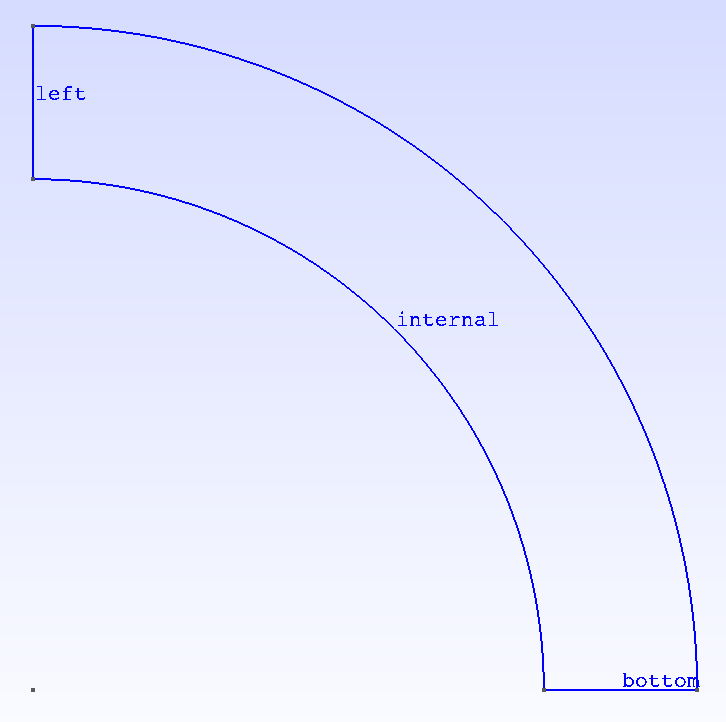
\includegraphics[width=0.7\linewidth]{img/geometry.png} \\ Geometry}
    \end{minipage}
    \hfill
    \begin{minipage}[h]{0.5\linewidth}
        \center{\includegraphics[width=0.9\linewidth]{img/plastic_strain.png} \\ Plastic strain on final load step}
    \end{minipage}
    \caption{Cylinder expansion problem}
    \label{fig:domain}
\end{figure}

In this particular case, the solution of the equilibrium problem of an elastic-plastic body can be found analytically. A detailed conclusion of a elastic-plastic model can be found in~\parencite{bonnet:hal-01083772}, and the implementation in the form of program code for Fenics 2019 is located on~\parencite{bleyer2018numericaltours}. Here we will limit ourselves to the relations already deduced
\begin{align}
    &\Delta p = 
    \begin{cases}
        \frac{1}{3\mu + H}, & \text{if } f_\text{elas} \geq 0,\\
        0, & \text{otherwise},
    \end{cases} \label{eqn:dp_von_mises}\\
    &\Delta\uusigma = \beta\uusn, \label{eqn:dsigma_von_mises}
\end{align}
where $\beta = \frac{3\mu}{\sigmaeqnelas}\Delta p$.

The stress derivative is written with the following formula
\begin{equation}
    \dfrac{\md\uusigman}{\md\uuDeltaeps} = \uuuuC{}_{n+1}^{\text{tang}} = \uuuuC{} - 3\mu \left( \frac{3\mu}{3\mu + H} -\beta \right) \uuN \otimes \uuN - 2\mu\beta\uuuuJ \label{eqn:C_tang_von_mises}
\end{equation}
where $\uuN = \frac{\uus}{\uusigmanelas}$.

So we can explicitly write out the linearization of the variational problem~\eqref{eqn:cylinder_var_1}--\eqref{eqn:cylinder_var_2}
\begin{align}
    & \text{Find } \Delta\uu \in V \text{ such that,} \label{eqn:cylinder_lin_var_from_1} \\ 
    & \int\limits_\Omega \left( \uuuuC{}_{n+1}^\text{tang} : \uueps(\Delta\uu) \right) : \uueps(\uv) \, \md x = -\int\limits_\Omega\uusigma_n : \uueps(\uv) \, \md x + q_{n+1}\int\limits_{\partial\Omega_\text{internal}}\un \cdot \uv \, \md x, \quad \forall \uv \in V. \label{eqn:cylinder_lin_var_from_2} 
\end{align}

Explicit expressions~\eqref{eqn:dp_von_mises}--\eqref{eqn:C_tang_von_mises} are possible thanks to the form of von Mises criterion~\eqref{eqn:cylinder_von_mises}. Similar expressions can be obtained for other criteria. As part of this work, a code has been written that allows to work with the plasticity of Drucker-Prager. A detailed derivation of similar expressions in this case can be found in the appendix section \ref{appendix:DP}.

Now we have at our disposal everything necessary for the successful modeling of the von Mises elasto-plasticity. In the next part, we will talk in detail about ways to solve this problem using various approaches via the FEniCSx and cvxpy libraries.

\subsection{Development}

The development of a program for modeling the cylinder expansion problem was carried out with the support of the finite element library FEniCSx. As mentioned earlier, the initial problem has different formulations, for each of which a separate program is written. The open source code is available on the Github repository~\cite{convex-plasticity}. 

In this section, we will talk about some nuances of modeling an elastic-plastic material using the FEniCSx library, as well as how to combine this modeling with other Python libraries that allow us to solve convex optimization problems.

\subsubsection{Voigt notation}

It is worth noting that the problems described above are formulated in terms of tensors of the second and fourth ranks, which complicates the development stage of the work. Taking into account the symmetry of the stress, strain and stiffness tensors, we propose to reformulate these problems of 2D plan in the Voigt notation.

According to this notation the stress tensor representation is a vector
\begin{equation*}
    \bsigma = (\sigma_{xx}, \sigma_{yy}, \sigma_{zz}, \sigma_{xy})^T,  
\end{equation*}
the strain one is a vector
\begin{equation*}
    \beps = (\varepsilon_{xx}, \varepsilon_{yy}, \varepsilon_{zz}, \varepsilon_{xy})^T,
\end{equation*}
where the shear components $xy$ of vectors $\bsigma$ and $\beps$ must be multiplied by $\sqrt{2}$ for some tasks where the correct calculation of such expressions as $\uusigma:\uueps$, $\uus:\uus$, etc is required. Other tensors, for example, deviatoric parts $\bs$ and $\be$ follow the same notation logic. The stiffness matrix of linear elasticity is 
\begin{equation*}
    \bC = 
    \begin{pmatrix}
        \lambda + 2\mu & \lambda & \lambda & 0 \\
        \lambda & \lambda + 2\mu & \lambda & 0 \\
        \lambda & \lambda & \lambda + 2\mu & 0 \\
        0 & 0 & 0 & 2\mu 
    \end{pmatrix}.
\end{equation*}
For simplicity, we will also highlight the vectors in bold.

Thus we rewrite in the Voigt notation the weak formulation of the cylinder expansion problem~\eqref{eqn:cylinder_var_1}--\eqref{eqn:cylinder_var_2}:
\begin{align}
    & \text{Find } \bu_{n+1} \in V \text{ such that,} \label{eqn:var_disc_from_1_voigt} \\ 
    & R(\bu_{n+1}) = \int\limits_\Omega\bsigma_{n+1} \cdot \beps(\bv) \, \md x - q_{n+1}\int\limits_{\partial\Omega_\text{internal}}\bn \cdot \bv \, \md x = 0, \quad \forall \bv \in V \label{eqn:var_disc_from_2_voigt},
\end{align}
where $\bsigma_{n+1} = \bsigma(\bu_{n+1})$ implicitly depends on $\bu_{n+1}$, and its linearized version~\eqref{eqn:cylinder_lin_var_from_1}--\eqref{eqn:cylinder_lin_var_from_2}:
\begin{align}
    & \text{Find } \Delta\bu \in V \text{ such that,} \label{eqn:cylinder_lin_var_1_voigt} \\ 
    & \int\limits_\Omega \left(\bC_{n+1}^\text{tang} \, \Delta\beps\right) : \beps(\bv) \, \md x = -\int\limits_\Omega\bsigma_n \cdot \beps(\bv) \, \md x + q_{n+1}\int\limits_{\partial\Omega_\text{internal}}\bn \cdot \bv \, \md x \label{eqn:cylinder_lin_var_2_voigt},
\end{align}
where $\bC_{n+1}^{\text{tang}}$ is a the tangent stiffness matrix and $\Delta\beps = \beps(\Delta\bu)$.

% \begin{equation}
%     \int\limits_\Omega\bsigma_{n+1}(\Delta\bu)\beps(\bv) \, \md x - q_{n+1}\int\limits_{\partial\Omega_\text{internal}}\bn \cdot \bv \, \md x = 0, \quad \forall \bv \in V,
% \end{equation}
% where 

% \begin{equation}
%     \int\limits_\Omega \left( \bC_{\text{tang}} \, \beps(\Delta\bu) \right) \cdot \beps(\bv) \, \md x - q_{n+1}\int\limits_{\partial\Omega_\text{internal}}\bn \cdot \bv \, \md x = 0, \quad \forall \bv \in V.
% \end{equation}

The convex optimization problem~\eqref{eqn:conic_problem} in Voigt notation is
\begin{equation}
    \label{eqn:conic_problem_Voigt}
    \begin{cases}
        \min\limits_{\bsigma, p} F(\bsigma, p), \\
        f(\bsigma, p) \leq 0,
    \end{cases}
\end{equation}
where the free energy $F$ of an elastoplastic material is expressed as follows
\begin{equation}
    F(\bsigma, p) = \frac{1}{2}(\bsigma_{n+1}^\text{elas} - \bsigma)^T \bS (\bsigma_{n+1}^\text{elas} - \bsigma) + \frac{1}{2}H(p_{n+1}^\text{elas} - p)^2,
\end{equation}
where $\bS$ is an inverted stiffness matrix.

\subsubsection{Stress tensor values}

Solving the equilibrium problem of an elastic-plastic solid, we find the values of the displacement vector at each node of the finite element mesh. To find the stress field, we need to calculate the derivative of the displacements. The displacements are defined in a second-order continuous Galerkin space, which does not guarantee the continuity of the first derivative at the mesh nodes. A common strategy for calculating stresses is an approach in which the values of the first derivatives of displacements are calculated at the Gauss points of each element. FEniCSx has the necessary functionality to implement this strategy. 

There is an entity \mypython{fem.Expression}, which represents a mathematical expression based on UFL package. It can contain a global coefficients \mypython{fem.Function}, another essential brick of FEniCSx. The last one represents global finite vectors such as the displacement one. Such coefficients are based on a finite element space: continuous Galerkin, discontinuous Galerkin, quadrature and others. There is an example below where finite element spaces and variables associated with them are initiated.

\begin{pythoncode}
    deg_u = 2
    deg_stress = 2
    V = fem.VectorFunctionSpace(mesh, ("CG", deg_u))
    We = ufl.VectorElement("Quadrature", mesh.ufl_cell(), degree=deg_stress, dim=4, quad_scheme='default')
    W = fem.FunctionSpace(mesh, We)

    u = fem.Function(V, name="Total_displacement")
    du = fem.Function(V, name="Iteration_correction")
    Du = fem.Function(V, name="Current_increment")
    sig = fem.Function(W, name="Current_stress")
\end{pythoncode}
Note that the stress vector \mypython{sig} is defined on the quadrature space, i.e. the values of the stress vector are stored in Gaussian nodes. 

To efficiently calculate stresses using FEniCSx tools, it is required to use the \mypython{eval} method of the entity \mypython{fem.Expression}, which interpolates the mathematical expression of stresses in Gaussian nodes. For ours purposes we wrote the function \mypython{interpolate_quadrature}, which implements this idea.The code below is an example of calculating the stress vector for the whole domain.
\begin{pythoncode}
    deps = eps(Du)
    sig_, N_, beta_, dp_ = proj_sig(deps, sig_old, p)
    fs.interpolate_quadrature(sig_, sig)
\end{pythoncode}
where \mypython{Du} is a solution on a current loading step, the function \mypython{eps} defines the mathematical expression of the strain tensor and the function \mypython{proj_sig} performs the return-mapping algorithm.

\subsubsection{Newton solvers}
To solve a nonlinear equation in the form~\eqref{eqn:var_from_1}--\eqref{eqn:var_from_2}, the Newton method is traditionally used, where the calculation of the objective function derivative is required. In this paper, three types of implementation of this method are used.

For those cases when we can find the stress derivative analytically, we use our own "naive" Newton method, which is implemented through the simplest loop, as well as using the SNES solver from the petsc library. 

In this paper, we are dealing with plasticity problems for which calculating the stress derivative analytically is problematic. That is why we also use the quasi-Newton method, which numerically approximates the derivative of the objective function, which means we do not need to know its explicit expression. This study uses an implementation of this algorithm in the form of SNESQN solver from the petsc library.

We would like to note here that the exact calculation of the derivative significantly affects the convergence of Newton methods, especially at the stages, where plastic deformations occur, therefore, to speed up the calculations, the original problem is solved in a dimensionless form. In this case, it is enough to change the input parameters, for example, as follows
\begin{align*}
    & E^* = \frac{E}{E} = 1, \quad \sigma_0^* = \frac{\sigma_0}{E}, \\
    & R_i^* = \frac{R_i}{R_i} = 1, \quad R_e^* = \frac{R_e}{R_i},
\end{align*}
where $E^*$, $\sigma_0^*$, $R_i^*$ and $R_e^*$ are dimensionless Young modulus, uniaxial strength, internal and external radii of the cylinder respectively.

\subsubsection{Classical approach}

In this section, we will describe main components of elastic-plastic modeling for solving the~\eqref{eqn:cylinder_var_1}--\eqref{eqn:cylinder_var_2} problem using FEniCSx. Only important parts of the program code will be given here. The full software implementation is made publicly available by~\parencite{convex-plasticity}. We recall that this implementation is based on the one of~\textcite{bleyer2018numericaltours}, where the von Mises plasticity analysis used the previous version of FEniCS 2019. The current version of FEniCSx 0.3.1.0 currently contains more features that allow us to improve the previous implementation. We call this approach \textit{classical} to pay tribute to the original implementation: the approach described here uses the same idea of determining the stress field $\uusigman$, the internal variable $p_{n+1}$ and other auxiliary variables in quadrature functional spaces. In this sense, the classical approach does not bring anything new, but optimizes the source code using the interpolation feature integrated into the \mypython{eval} method of \mypython{fem.Expression} entity.

To initialize target variables and function spaces, it is enough to write the following lines of code:

\begin{pythoncode}
    deg_u = 2
    deg_stress = 2
    V = fem.VectorFunctionSpace(mesh, ("CG", deg_u))
    We = ufl.VectorElement("Quadrature", mesh.ufl_cell(), degree=deg_stress, dim=4, quad_scheme='default')
    W = fem.FunctionSpace(mesh, We)
    W0e = ufl.FiniteElement("Quadrature", mesh.ufl_cell(), degree=deg_stress, quad_scheme='default')
    W0 = fem.FunctionSpace(mesh, W0e)

    u = fem.Function(V, name="Total_displacement")
    du = fem.Function(V, name="Iteration_correction")
    Du = fem.Function(V, name="Current_increment")
    sig = fem.Function(W, name="Current_stress")
    N = fem.Function(W)
    beta = fem.Function(W0)
    p = fem.Function(W0, name="Cumulative_plastic_strain")
    dp = fem.Function(W0)
\end{pythoncode}

It can be seen from this code that we store the values of $\uusigman$ in a vector \mypython{sig} ($\bsigma_{n+1}$ in Voigt notation). In the future, we will work with $\uusigman$ in both tensor and Voigt notations, depending on convenience.

In this approach, we use our own custom Newton method. It means that we need to define a linearized variational problem~\eqref{eqn:cylinder_lin_var_from_1}--~\eqref{eqn:cylinder_lin_var_from_2} using FEniCSx tools. So we have to represent $\uuuuC{}_{n+1}^\text{tang}$ as \mypython{fem.Expression} using UFL. Although FEniCSx allows us to work with rank 4 tensors, in this case it is more convenient to work with the expression $\uuuuC{}_{n+1}^\text{tang} : \uueps(\Delta\uu)$ and not to store the values of the entire tensor $\uuuuC{}_{n+1}^\text{tang}$ globally, so we use the function \mypython{sigma_tang} 
\begin{pythoncode}
    def sigma_tang(e):
    N_elas = as_3D_tensor(n_elas)
    return sigma(e) - 3*mu*(3*mu/(3*mu+H)-beta)*ufl.inner(N_elas, e)*N_elas - 2*mu*beta*ufl.dev(e)  
\end{pythoncode}
to define a weak formulation as follows
\begin{pythoncode}
    u_ = ufl.TrialFunction(V)
    v_ = ufl.TestFunction(V)
    a_Newton = ufl.inner(sigma_tang(eps(v_)), eps(u_))*dx
    res = -ufl.inner(eps(v_), as_3D_tensor(sig))*dx + F_ext(v_)
    my_problem = pf.LinearProblem(a_Newton, res, Du, bcs)
\end{pythoncode}
The return-mapping procedure is performed using the \mypython{proj_sig} function
\begin{pythoncode}
    def proj_sig(deps, old_sig, old_p):
        sig_n = as_3D_tensor(old_sig)
        sig_elas = sig_n + sigma(deps)
        s = ufl.dev(sig_elas)
        sig_eq = ufl.sqrt(3/2.*ufl.inner(s, s))
        f_elas = sig_eq - sig0 - H*old_p
        dp = ppos(f_elas)/(3*mu+H)
        n_elas = s/sig_eq*ppos(f_elas)/f_elas
        beta = 3*mu*dp/sig_eq
        new_sig = sig_elas-beta*s
        return ufl.as_vector([new_sig[0, 0], new_sig[1, 1], new_sig[2, 2], new_sig[0, 1]]), \
            ufl.as_vector([n_elas[0, 0], n_elas[1, 1], n_elas[2, 2], n_elas[0, 1]]), \
            beta, dp       
\end{pythoncode}

It accepts a \mypython{fem.Expression} object \mypython{deps} as input, as well as global vectors \mypython{old_sig} and \mypython{old_p} (stress and plastic strain values) from the previous loading step. It returns 4 \mypython{fem.Expression} objects, each of which is a combination of mathematical formulas based on the UFL functional and the \mypython{du} coefficient. The latter is a global vector of displacements increment on a current Newton iteration.

Using the \mypython{interpolate_quadrature} function, we calculate the values of these expressions at each Gaussian node and update the \mypython{sig}, \mypython{N} and \mypython{beta} variables. We have to save the last two globally, since they are necessary for the \mypython{sigma_tang} function. Thus, we update the variational formulation also.
\begin{pythoncode}
    deps = eps(Du)
    sig_, N_, beta_, dp_ = proj_sig(deps, sig_old, p)
    fs.interpolate_quadrature(sig_, sig)
    fs.interpolate_quadrature(N_, N)
    fs.interpolate_quadrature(beta_, beta)
\end{pythoncode}

Before moving on to convex plasticity approach, we would like to talk about another way to implement the classical one. The fact is that we can differentiate UFL expressions using the \mypython{ufl.derivative} function. If we can write down a weak formulation~\eqref{eqn:cylinder_var_1}--\eqref{eqn:cylinder_var_2}, then we could use external Newton methods (for example, SENS from the \mypython{petsc} library) and pass them the derivative $R^\prime(\uu)$ instead of calculating it manually by finding the $\uuuuC{}_{n+1}^\text{tang}$ expression. To do this, it is necessary to rewrite the original variational problem in the following form
\begin{align}
    & \text{Find } \uu \text{ such that} \label{eqn:cylinder_SNES_var_1} \\
    & R = \int\limits_\Omega \uusigman : \uueps(\uv) \, \md\Omega - \uF_{n+1}^\text{ext} = \int\limits_\Omega \left( \uusigma_n + \uuuuC{} : (\Delta\uueps - \Delta\uueps^p) \right) : \uueps(\uv) \, \md\Omega - \uF_{n+1}^\text{ext} = 0, \label{eqn:cylinder_SNES_var_2}
\end{align}
where $\Delta\uueps = \uueps(\Delta\uu)$ and the plastic deformation increment $\Delta\uueps^p = \uueps^p(\Delta\uu)$ actually contains a return-mapping algorithm inside. Explicitly it can be written out as follows
\begin{equation}
    \Delta\uueps^p = 
        \begin{cases}
            \Delta p \left( \frac{3}{2}\frac{\uusnelas} {\sigmaeqnelas} \right), & \text{ if } f(\uusigmanelas, p_n) > 0,  \\
            0, & \text{ otherwise}.
        \end{cases}
\end{equation}
In terms of FEniCSx code should be written as follows:
\begin{pythoncode}
    def deps_p(deps, old_sig, old_p):
        sig_n = as_3D_tensor(old_sig)
        sig_elas = sig_n + sigma(deps)
        s = ufl.dev(sig_elas)
        sig_eq = ufl.sqrt(3/2.*ufl.inner(s, s))
        f_elas = sig_eq - sig0 - H*old_p
        dp_sig_eq = ufl.conditional(f_elas > 0, f_elas/(3*mu+H)/sig_eq, 0) 
        return 3./2. * dp_sig_eq * s 
\end{pythoncode}
Then we can define a new variational problem and its solver:
\begin{pythoncode}
    residual = ufl.inner(as_3D_tensor(sig) + sigma(eps(Du) - deps_p(eps(Du), sig, p)), eps(u_))*dx - F_ext(u_)
    J = ufl.derivative(ufl.inner(sigma(eps(Du) - deps_p(eps(Du), sig, p)), eps(u_))*dx, Du, v)
    my_problem = pf.SNESProblem(residual, Du, J, bcs, petsc_options=petsc_options_SNES)
\end{pythoncode}
where \mypython{pf.SNESProblem} is a support class to work with the SNES solver.

We note here that, as in the classical approach, this method is possible only in special cases when it is possible to calculate analytically $\Delta\uueps^p$.

\subsubsection{Convex plasticity}
We call the \textit{convex plasticity} or the convex optimization approach the one where the return-mapping algorithm is implemented by solving the optimization problem. It is solved at some point in the domain where we know the values of the stress components and cumulative plastic strain. We noted above that the stresses are calculated in Gaussian nodes, so the problem must be solved in each individual node. This approach is not numerically efficient. It is more convenient to solve it simultaneously for several Gaussian nodes. In this case, the order is not important. Therefore, we need to reformulate the problem~\eqref{eqn:conic_problem_Voigt} in vector form. 

For this purpose, we will assemble several Gauss nodes into groups or patches. If there are $N_q$ Gauss points in total in a functional space of quadratures, then there will be $1 \leq N_\text{patch} \leq N_q$ points in one patch. Using this notation, we will rewrite the conic optimization problem in vector~\eqref{eqn:conic_problem_Voigt} form:
\begin{equation}
    \label{eqn:conic_problem_vectorized}
    \begin{cases}
        \min\limits_{\bSigma, \bP} F(\bSigma, \bP), \\
        \mathbold{f}(\bSigma, \bP) \leq 0,
    \end{cases}
\end{equation}
where the vector $\bSigma$ with the size $4*N_\text{patch}$ contains sequentially 4 components of the stress vector $\bsigma$ for $N_\text{patch}$ Gauss nodes. By analogy, vectors $\bP$ and $\mathbold{f}$ contain cumulative plastic strain $p$ and yield criterion $f$ values respectively for $N_\text{patch}$ Gauss nodes. Then, keeping the previous notation, the free energy $F$ will be written in the following form 
\begin{equation}
    F(\bSigma, \bP) = \frac{1}{2}(\bSigma_{n+1}^\text{elas} - \bSigma)^T \mathbb{S} (\bSigma_{n+1}^\text{elas} - \bSigma) + \frac{1}{2}H(\bP_{n+1}^\text{elas} - \bP)^T(\bP_{n+1}^\text{elas} - \bP),
\end{equation}
where the matrix $\mathbb{S}$ with the size $4*N_\text{patch}\times4*N_\text{patch}$ is the block-diagonal matrix with the inverted stiffness matrix $\bS$ on its diagonal.

In order to solve this problem numerically, we use the \mypython{cvxpy} library. It allows to use various third-party conve solvers, for instance, SCS, MOSEK and ECOS were used in this work. For convenience the \mypython{ReturnMapping} class is written, which formulates the problem using the \mypython{cvxpy} library and finds its numerical solution.

Note that the free energy $F$ doesn't depend on the plasticity criterion. In order to change the plasticity model, it is enough to change the constraint of the optimization problem~\eqref{eqn:conic_problem_vectorized}. This makes the convex plasticity approach more general compared to the classical one. In this regard, it is impossible to know in advance the stress derivative, which is necessary for the Newton method, so we use the quasi-Newton one here. As a result, the algorithm of the convex plasticity approach consists of the following steps:
\begin{itemize}
    \item We consider the problem in the weak formulation~\eqref{eqn:cylinder_var_1}--\eqref{eqn:cylinder_var_2}.
    \item We use the SNESQN \mypython{petsc} to solve it.
    \item During each quasi-Newton iteration we carry out the projection of $\bsigma^\text{elas}_{n+1}$ on the yield surface, solving the vectorized optimization problem~\eqref{eqn:conic_problem_vectorized}.
\end{itemize}
Note that the optimization problem is solved $\left\lfloor N_q / N_\text{patch}\right\rfloor$ times, if this division contains a nonzero remainder, then the conic problem~\eqref{eqn:conic_problem_vectorized} is solved additionally for the remaining $N_q \bmod N_\text{patch}$ Gauss points. 

\subsection{Performance}

The second part of this paper discusses strategies to improve the performance of the described above approaches solving plasticity problems. Before describing these ones in detail, we will first talk about the obstacles, that we encountered during the development of the methods presented in the first part of this research. 

% In the particular case of modeling an elastic-plastic material defined by the von Mises yield criterion, we explicitly wrote down the variational formulation of. is the dependence is nonlinear in nature

Let's return to a general non-linear variational problem~\eqref{eqn:var_from_1}--\eqref{eqn:var_from_2}. Obviously, the case of modeling an elastic-plastic material defined by the von Mises yield criterion, is just an example where UFL features are sufficient to solve the problem. There are other models where the stress tensor $\uusigma$ is difficult to represent explicitly. Let us show you some others examples

\begin{itemize}
    % \item[$\bullet$] $\uusigma = \uuuuC{} : (\uueps - \uueps^p)$
    \item[$\bullet$] $\uusigma(\underline{u}) = f(\varepsilon_\text{I}, \varepsilon_\text{II}, \varepsilon_\text{III})$,
    \item[$\bullet$] $\uusigma(\underline{u}) = \underset{\alpha}{\operatorname{argmin}}\, g(\underline{\underline{\varepsilon}}(\underline{u}),  \alpha)$,
\end{itemize}
where $\varepsilon_\text{I}, \varepsilon_\text{II}, \varepsilon_\text{III}$ are eigenvalues of $\underline{\underline{\varepsilon}}$ and $g$ is some scalar function.

% In addition to the above, we note that the convex plasticity approach could also be implemented in the assembly process 

% Find $\underline{u} \in V$, such that

% $$ F(\underline{u}) = \int_\Omega \uusigma(\underline{u}) : \underline{\underline{\varepsilon}}(\underline{v}) dx - \int_\Omega \underline{f} \underline{v} dx = 0 \quad \forall \underline{v} \in V,$$
% where an expression of $\underline{\underline{\sigma}}(\underline{u})$ is non linear and cannot be defined via UFL. Let us show you some examples

As seen in the second example, $\uusigma(\underline{u})$ can also implicitly depend on the value of other scalar, vector or even tensorial quantities ($\alpha$ here). The latter do not necessarily need to be represented in a finite-element function space. They shall just be computed during the assembling procedure when evaluating the expression $\uusigma(\underline{u})$ pointwise.

Although we use the quasi-Newton method to find the solution of~\eqref{eqn:cylinder_var_1}--\eqref{eqn:cylinder_var_2}, which allows us to bypass the exact calculation of the derivative of $\uusigma$ with respect to $\underline{u}$, we would like to have a more reliable way to solve the problem in the case when we know the expression of the derivative (as, for example, it is so for von Mises and Drucker-Prager plasticity models), but it is difficult to express it using UFL tools. Otherwise we have a method that is able to approximate the derivative more accurately (as, for example, the \mypython{derivative()} method of the cvxpy package does). Thus, it is necessary to have a functionality which will allow to do a simultaneous calculation of $\uusigma$ and its derivative during assembling procedure regardless of the calculation method.

% In both cases, custom assembling would significantly speed up calculations.

In addition to the inconveniences described above, we are faced with the problem of excessive memory allocation. For example, in the classic approach we are forced to save global variables $\beta$ and $\bN$. If there is a mesh containing $N_\text{elements}$ elements, we have to allocate memory for a vector with the size $N_\text{elements}*3$ for the scalar field $\beta$ from \mypython{W0} finite space and another one with the size $N_\text{elements}*3*4$ for the vector field $\bN$ from \mypython{W} finite space. At the same time they are intermediate variables, necessary only for the calculation of the stress tensor and its derivative. So we would like to avoid such a waste of memory.

% \todounderline{Write about global Ctang?}

% In addition, in order to use a standard Newton method to find the solution of $F(\underline{u})=0 $, we also need to compute the derivative of $\uusigma $ with respect to $\underline{u} $. The latter may also depend on some internal variables $\alpha $ of $\uusigma $. Thus, it is necessary to have a fonctionality which will allow to do a simultaneous calculation of $\uusigma$ and its derivative during assembling procedure.

% In practice, in the previous examples $\ \uusigma $ depends directly on $\ \underline{\underline{\varepsilon}} = \frac{1}{2}(\nabla \underline{u} + \nabla \underline{u}^T) $. As a result, it is more natural to consider the non-linear expression as a function of $\ \underline{\underline{\varepsilon}} $ directly, provide an expression for $\ \dfrac{d\uusigma}{d\underline{\underline{\varepsilon}}} $ and evaluate $\ \dfrac{d\uusigma}{d\underline{u}} $ by the chain rule (letting UFL handle the $\ \dfrac{d\underline{\underline{\varepsilon}}}{d\underline{u}} $ part).

As the result we require the following features to increase capabilities of the code implemented in the first part of this project:
\begin{enumerate}
    \item To define nonlinear expressions of variational problems in more complex way than it's allowed by UFL
    \item To let an "oracle" provide values of such an expression and its derivative(s)
    \item To call this oracle on-the-fly during the assembly to avoid unnecessary loops, precomputations and memory allocations
\end{enumerate}

Next sections describe our own view of these features implementation.

\subsubsection{Custom assembling}

Following the concept of the custom assembler~\parencite{test_custom_assembler}, which uses the power of \mypython{numba} and \mypython{cffi} python libraries, we implemented our own version of custom assembler, where we can change the main loop of the assembling procedure.

There are several essential elements of the algorithm to be mentioned. First of all, we would like to introduce a concept of \mypython{CustomExpression}, which is essential for our study. Let us consider the next simple variational problem 
$$ \int_\Omega g \uu \cdot \uv dx, \quad \forall \underline{v} \in V, $$
where $\underline{u}$ is a trial function, $\underline{v}$ is a test function and the function $g$ is a mathematical expression. For this moment we must use \mypython{fem.Function} class to implement this variational form. Knowing the exact UFL expression of $g$ we can calculate its values on every element using the interpolation procedure of \mypython{fem.Expression} class. So we save all values of $g$ in one global vector. The goal is to have a possibility to calculate the expression $g$, no matter how difficult it is, in every element node (for instance, in every gauss point, if we define $g$ on a quadrature element) during the assembling procedure. So, we introduce a new entity named as \mypython{CustomExpression}. It
\begin{enumerate}
    \item inherits \mypython{fem.Function}
    \item contains a method \mypython{eval}, which will be called inside of the assemble loop and calculates the function local values
\end{enumerate}

Besides \mypython{CustomExpression} we need an other entity. Every \mypython{fem.Function} object stores its values globally, but we would like to avoid such a waste of memory updating the function value during the assembling procedure. Let us consider the previous variational form, where $g$ contains its local-element values now. If there is one local value of $g$ (only 1 gauss point), the use of the \mypython{fem.Constant} entity would be enough, but it is a particular case. In general, we are dealing with quadrature functional spaces of arbitrary degree (for example, \mypython{W0} or Q2 space from the first part). We need to store different local values of $g$ in every gauss point. So we introduce a concept of \mypython{DummyFunction} (or `ElementaryFunction`?), which 
\begin{enumerate}
    \item inherits \mypython{fem.Function}
    \item allocates the memory for local values only
    \item can be updated during assembling procedure
\end{enumerate}

\subsubsection{Examples}

We implemented an elasticity problem to explain our ideas by simple example. Let's consider a beam stretching with the left side fixed. On the other side we apply displacements. 
\begin{align}
    & \text{Find } \underline{u} \in V \text{ s.t.} \\
    & \int_\Omega \uusigma(\underline{\underline{\varepsilon}}(\underline{u})) : \underline{\underline{\varepsilon}}(\underline{v}) d\underline{x}  = 0 \quad \forall \underline{v} \in V,
\end{align}
with following boundary conditions
\begin{align}
    & (0, 0) : u_y = 0, \\
    & \partial\Omega_\text{left} : u_x = 0, \\
    & \partial\Omega_\text{right} : u_x = t \cdot u_\text{bc},
\end{align}
where $u_\text{bc}$ is a maximal displacement on the right side of the beam, $t$ is a parameter varying from 0 to 1, and where $\uusigma(\underline{\underline{\varepsilon}})$ is our user-defined "oracle". Here we use a simple elastic behaviour:
\begin{equation}
    \uusigma(\underline{\underline{\varepsilon}}) = \uuuuC{}:\underline{\underline{\varepsilon}},
\end{equation}
and for which the derivative is:
\begin{equation}
    \dfrac{d\uusigma}{d\underline{\underline{\varepsilon}}} = \uuuuC{}.
\end{equation}

Let's focus on the key points. In this "naive" example the derivative is constant, but in general non-linear models, its value will directly depend on the local value of $\underline{\underline{\varepsilon}}$. We would like to change this value at every assembling step and to avoid additional memory allocation. As it's the stress tensor derivative, it's defined on quadrature elements. Thus, in our terms, it would be a \mypython{DummyFunction}. Obviously, $\uusigma$ is the \mypython{CustomExpression}, which depends on $\underline{\underline{\varepsilon}}$. 

The code below initiates variables associated with $\uuuuC{}$ and $\uusigma$ respectively:
\begin{pythoncode}
    q_dsigma = ca.DummyFunction(VQT, name='stiffness') # tensor C
    q_sigma = ca.CustomExpression(VQV, eps(u), [q_dsigma], get_eval)  # sigma_{n+1}
\end{pythoncode}

In the \mypython{CustomExpression} constructor we observe three arguments. The first one is the UFL-expression of its variable ($\uueps$ here). It will be compiled via \mypython{ffcx} and will be sent as "tabulated" expression to a numba (compilable) function, which performs the calculation of \mypython{q_sigma}. The second argument is a list of \mypython{q_sigma} coefficients (\mypython{fem.Function} or \mypython{DummyFunction}), which takes a part in calculations of \mypython{q_sigma}. The third argument contains the function \mypython{get_eval} generating a \mypython{CustomExpression} method \mypython{eval}, which will be called during the assembling. It describes every step of local calculation of $\uusigma$. In this linear elasticity example it simply multiplies the stiffness tensor $\bC$ and the strain vector $\beps$:

\begin{pythoncode}
    def get_eval(self:ca.CustomFunction):
        tabulated_eps = self.tabulated_input_expression
        n_gauss_points = len(self.input_expression.X)
        local_shape = self.local_shape
        C_shape = self.stiffness.shape

        @numba.njit(fastmath=True)
        def eval(sigma_current_local, coeffs_values, constants_values, coordinates, local_index, orientation):
            epsilon_local = np.zeros(n_gauss_points*3, dtype=PETSc.ScalarType)

            C_local = np.zeros((n_gauss_points, *C_shape), dtype=PETSc.ScalarType)
            
            sigma_local = sigma_current_local.reshape((n_gauss_points, *local_shape))

            tabulated_eps(ca.ffi.from_buffer(epsilon_local), 
                        ca.ffi.from_buffer(coeffs_values), 
                        ca.ffi.from_buffer(constants_values), 
                        ca.ffi.from_buffer(coordinates), ca.ffi.from_buffer(local_index), ca.ffi.from_buffer(orientation))
            
            epsilon_local = epsilon_local.reshape((n_gauss_points, -1))

            for q in range(n_gauss_points):
                C_local[q][:] = get_C() #change DummyFunction here
                sigma_local[q][:] = np.dot(C_local[q], epsilon_local[q]) 
            
            sigma_current_local[:] = sigma_local.flatten()

            
            return [C_local.flatten()]
        return eval
\end{pythoncode}

Besides the local implementation of new entities we need to change the assembling procedure loop to describe explicitly the interaction between different coefficients of linear and bilinear forms. It allows us to write a quite general custom assembler, which will work for any kind non-linear problem. Thus we have to define two additional numba functions to calculate local values of forms kernels coefficients (see the code below).

\begin{pythoncode}
    @numba.njit(fastmath=True)
    def local_assembling_b(cell, coeffs_values_global_b, coeffs_coeff_values_b, coeffs_dummy_values_b, coeffs_eval_b, 
                           u_local, coeffs_constants_b, geometry, entity_local_index, perm):
        sigma_local = coeffs_values_global_b[0][cell]
        
        output_values = coeffs_eval_b[0](sigma_local, 
                                         u_local, 
                                         coeffs_constants_b[0], 
                                         geometry, entity_local_index, perm)
    
        coeffs_b = sigma_local
    
        for i in range(len(coeffs_dummy_values_b)):
            coeffs_dummy_values_b[i][:] = output_values[i] #C update
    
        return coeffs_b
    
    @numba.njit(fastmath=True)
    def local_assembling_A(coeffs_dummy_values_b):
        coeffs_A = coeffs_dummy_values_b[0]
        return coeffs_A
\end{pythoncode}

With this "naive" example, we demonstrated the possibility of intervention in the assembly process with ready-made FEniCSx tools, and with the help of compiled functions of the numba library. The implementation of the proposed functionality is effective enough not to change the source code of the FEniCSx library itself.

The following example optimizes the classical approach solving the von Mises plasticity problem:~\eqref{eqn:cylinder_var_1}--\eqref{eqn:cylinder_var_2}.
% Plasticity problem
% The elasticity case is trivial and doesn't show clearly our demands by the described above features. Therefore we present here a standard non-linear problem from our scientific domain - a plasticity one.
% The full description of the problem and its implementation on a legacy version of FEniCS 2019 is introduced [here] \todolink. Note that for this very specific example, everything can still be expressed in UFL directly. However, in general, this is no longer the case, as one may have to solve a nonlinear equation at each integration point to obtain the expression of stresses and plasticity variables.
% We focus on the following variational problem only: Find $\underline{\Delta u} \in V$ s.t.
% $$ \int\limits_\Omega \underline{\underline{\sigma_{n+1}}} (\underline{\underline{\varepsilon}}(\underline{\Delta u})) : \underline{\underline{\varepsilon}}(\underline{v}) dx - q \int\limits_{\partial\Omega_{\text{inside}}} \underline{n} \cdot \underline{v} dx = 0, \quad \forall \underline{v} \in V, $$
% where $\underline{\Delta u}$ is a displacement increment between two load steps, $\uusigma_{n+1}$ is the current stress tensor which depends on the previous stress $\uusigma_n$ and the previous plastic strain $p_n$ and which is implicitly defined as the solution to the following equations:
We can conclude from this, that the fields $\underline{\underline{\sigma_{n+1}}} = \underline{\underline{\sigma_{n+1}}}(\underline{\underline{\Delta\varepsilon}}, \beta, \uuN, dp, p_n, \underline{\underline{\sigma_n}})$ and $\mathbf{C}^\text{tang} = \mathbf{C}^\text{tang}(\beta, \uuN)$ depend on the common variables $\beta$ and $\uuN$. With the previous implementation, it was necessary to allocate additional space for them and calculate $\underline{\underline{\sigma_{n+1}}}$ and $\mathbf{C}^\text{tang}$ separately, but now we can combine their local evaluations.

In comparison with the elasticity case the \mypython{CustomExpression} \mypython{sig} has more dependent fields. Look at the code below

\begin{pythoncode}
    C_tang = ca.DummyFunction(QT, name='tangent') # tensor C_tang
    sig = ca.CustomExpression(W, eps(Du), [C_tang, p, dp, sig_old], get_eval) # sigma_n
\end{pythoncode}
As it was expected, the local evaluation of the \mypython{CustomExpression} becomes more complex 
\begin{pythoncode}
    def get_eval(self:ca.CustomExpression):
        tabulated_eps = self.tabulated_input_expression
        n_gauss_points = len(self.input_expression.X)
        local_shape = self.local_shape
        C_tang_shape = self.tangent.shape

        @numba.njit(fastmath=True)
        def eval(sigma_current_local, sigma_old_local, p_old_local, dp_local, 
                 coeffs_values, constants_values, coordinates, local_index, orientation):
            deps_local = np.zeros(n_gauss_points*3*3, dtype=PETSc.ScalarType)
            
            C_tang_local = np.zeros((n_gauss_points, *C_tang_shape), dtype=PETSc.ScalarType)
            
            sigma_old = sigma_old_local.reshape((n_gauss_points, *local_shape))
            sigma_new = sigma_current_local.reshape((n_gauss_points, *local_shape))

            tabulated_eps(ca.ffi.from_buffer(deps_local), 
                          ca.ffi.from_buffer(coeffs_values), 
                          ca.ffi.from_buffer(constants_values), 
                          ca.ffi.from_buffer(coordinates), 
                          ca.ffi.from_buffer(local_index), 
                          ca.ffi.from_buffer(orientation))
            
            deps_local = deps_local.reshape((n_gauss_points, 3, 3))

            n_elas = np.zeros((3, 3), dtype=PETSc.ScalarType) 
            beta = np.zeros(1, dtype=PETSc.ScalarType) 
            dp = np.zeros(1, dtype=PETSc.ScalarType) 

            for q in range(n_gauss_points):
                sig_n = as_3D_array(sigma_old[q])
                sig_elas = sig_n + sigma(deps_local[q])
                s = sig_elas - np.trace(sig_elas)*I/3.
                sig_eq = np.sqrt(3./2. * inner(s, s))
                f_elas = sig_eq - sig0 - H*p_old_local[q]
                f_elas_plus = ppos(f_elas)
                dp[:] = f_elas_plus/(3*mu_+H)
                
                sig_eq += TPV # for the case when sig_eq is equal to 0.0
                n_elas[:,:] = s/sig_eq*f_elas_plus/f_elas
                beta[:] = 3*mu_*dp/sig_eq
        
                new_sig = sig_elas - beta*s
                sigma_new[q][:] = np.asarray([new_sig[0, 0], new_sig[1, 1], new_sig[2, 2], new_sig[0, 1]])
                dp_local[q] = dp[0]
                
                C_tang_local[q][:] = get_C_tang(beta, n_elas)
            
            return [C_tang_local.flatten()] 
        return eval
\end{pythoncode}

Thus it can been seen more clearly the dependance of the tensor $\mathbf{C}^\text{tang}$ on the calculation of the tensor $\uusigma_{n+1}$. The full source code of this examples can be found in the \mypython{assembling_strategies} folder of the repository~\parencite{convex-plasticity}.

Finally we developed our own custom assembler which makes use of two new entities. This allows us to save memory, avoid unnecessary global *a priori* evaluations and do instead on-the-fly evaluation during the assembly. More importantly, this allows to deal with more complex mathematical expressions, which can be implicitly defined, where the UFL functionality is quite limited. Thanks to `numba` and `cffi` python libraries and some FEniCSx features, we can implement our ideas by way of efficient code. 
% Our realization doesn't claim to be the most efficient one. So, if you have any comments about it, don't hesitate to share them with us!

\newpage
\section{Results}
% \section{Résultats}

\subsection{Qualitative yield criterions comparison}

Here we compare various elastic-plastic models, plotting the displacements of the inner surface of the cylinder ($u_x(R_i, 0)$) at the end of the loading process. The final values of the movements are shown on the image~\ref{fig:yield_criteria}. These results are obtained thanks to the convex plasticity approach, based on solving the optimization problem and using the FEniCSx and cvxpy libraries.
\begin{figure}[H]
    \center
    \includegraphics[width=1\linewidth]{img/yield_criterions.png}
    \caption{Displacements of the inner boundary for different yield criteria using convex plasticity approach}
    \label{fig:yield_criteria}
\end{figure}
As we can see, the proposed approach gives correct results for all the criteria considered in this paper and various values of their parameters (for the Drucker-Prager criterion, we vary the parameter $\alpha$). This approach makes it possible to simulate the elastic-plastic behavior of the material, including that determined by the Rankine criterion. We recall that it is difficult to implement the classical approach in this case, especially in the three-dimensional one.

\subsection{Patch size effect on vectorized convex optimization problem}
The purpose of this work is not only to test the implementation of the convex plasticity approach in the form of ready-made program code, but also its effectiveness. If this implementation solves the task significantly slower than other approaches, then there will be insufficient benefits in it, especially if we are talking about complex three-dimensional problems. Therefore, we need to analyze the impact of solving the optimization problem using the cvxpy library on the overall simulation results. 

For numerical tests, the initial problem with the von Mises criterion was chosen as the target one, as well as 3 finite element meshes of different densities, the sizes of which are presented in the table below:

\begin{table}[H]
	\centering
	\begin{tabular}{|cccc|}
		\hline
		Mesh & Nodes & Elements & Gauss points of Q2 space \\
		\hline
		Coarse & 50	& 69 & 207 \\
		Medium & 407 & 714 & 2142 \\
		Dense & 811	& 1478 & 4434 \\
		\hline
	\end{tabular}
	\caption{Mesh data of time performance numerical tests for patch size effect}
    \label{tab:cvxpy_tests}
\end{table}
where Q2 space means the size of the finite element functional space of the second degree based on quadrature elements.

The images~\ref{fig:conic_solvers_coarse}--\ref{fig:conic_solvers_dense} demonstrate a comparison of the total program time for three meshes of different densities, using three different conic solvers depending on the patch size $N_\text{patch}$. The compilation time of the optimization problem was also measured. The fact is that before solving a problem formulated in the form of \eqref{eqn:conic_problem_vectorized} cvxpy converts it into a canonical form, which most conic solvers work with. For convenience, the plots from these images are duplicated on a logarithmic scale.

As can be seen from the plots, the larger the patch size, the longer it takes to compile using cvxpy. Starting from some point, this time is comparable to the total time of solving the conic problem. At the same time, with large values of $N_\text{patch}$, the compilation process consumes significantly RAM. That is why, for denser meshes, it is not possible to solve the problem for patch sizes equal to the total number of Gauss points in quadrature space defined on these meshes (components of the stress vector $\bsigma$ and cumulative plastic strain $p$ are defined in such spaces). Despite this, we can state that with an increase in the size of the patch, the time to solve the optimization problem decreases significantly. Starting from some $N_\text{patch}$, this decrease does not considerably affect the time of the program.

In addition, comparing conic solvers, we see that MOSEK solver works better than others with high-dimensional problems, but at the same time it's much worse with small-dimensional ones. SCS is comparable in time to MOSEK. The ECOS solver is slower to solve high-dimensional problems.

\begin{figure}[H]
    \center
    \includegraphics[width=1\linewidth]{img/conic_solvers_coarse.png}
    \caption{Patch size effect on the time performance of solving the conic problem: coarse mesh case}
    \label{fig:conic_solvers_coarse}
\end{figure}

\begin{figure}[H]
    \center
    \includegraphics[width=1\linewidth]{img/conic_solvers_medium.png}
    \caption{Patch size effect on the time performance of solving the conic problem: medium mesh case}
    \label{fig:conic_solvers_medium}
\end{figure}

\begin{figure}[H]
    \center
    \includegraphics[width=1\linewidth]{img/conic_solvers.png}
    \caption{Patch size effect on the time performance of solving the conic problem: dense mesh case}
    \label{fig:conic_solvers_dense}
\end{figure}

Summarizing the numerical tests described above, we can conclude the following:
\begin{itemize}
    \item The larger the patch size, i.e. the larger the dimension of the vectorized conic optimization problem, the faster the program runs.
    \item Starting with a certain patch size, the program is not significantly accelerated.
    \item For large patch sizes, cvxpy expends substantial computer resources to compile the optimization problem.
    \item For very dense meshes, it will not be possible to speed up the program by increasing the patch size.
    \item MOSEK works faster with problems of high dimension, but slower with small ones.
    \item ECOS is less suitable for high-dimensional problems.
    \item SCS is an optimal conic solver for problems of any dimension.
\end{itemize}

\subsection{Custom assembling performance}

In this section, we analyze the effectiveness of the implementation of the custom assembly approach regarding the classical one and depending on the mesh density. A series of numerical tests was performed based on the original cylinder expansion problem using the von Mises criterion. Each test corresponds to a finite element mesh, data of which are presented in the table~\ref{tab:custom_assembling_tests}. 

\begin{table}[H]
	\centering
	\begin{tabular}{|cccc|}
		\hline
		Mesh & Nodes & Elements & Gauss points of Q2 space \\
		\hline
		1 & 50	& 69 & 207 \\
		2 & 811 & 1478 & 4434 \\
		3 & 3706 & 7095 & 67707 \\
		4 & 11567 & 22569 & 67707 \\
		5 & 31666 & 62392 & 187176 \\
		\hline
	\end{tabular}
	\caption{Mesh data of time performance numerical tests of the custom assembling approach}
    \label{tab:custom_assembling_tests}
\end{table}

The figure~\ref{fig:custom_assembling_analysis} shows the dependence of the total running time of the program on different meshes (as the mesh number increases, its density increases as well). Using 'JIT overhead', we indicated the compilation time of python code written using the numba package.

\begin{figure}[H]
    \center
    \includegraphics[width=0.7\linewidth]{img/custom_assembling_tests.png}
    \caption{Time performance of the custom assembling approach in comparison with the classical one}
    \label{fig:custom_assembling_analysis}
\end{figure}

The results of the numerical experiment show that the compilation time of JIT overhead is an essential part of the total running time of the program for low-density meshes. At the same time, as the mesh density increases, the ratio of the compilation time to the total running time of the program tends to zero. This is possible due to the fact that the compilation of numba code occurs once during the first iteration of the Newton method. After that, the program uses the already compiled code throughout the entire modeling process.

From this we can conclude that for complex nonlinear problems, as well as those where the use of a mesh with a large number of elements is required, the compilation time is negligible compared with the total running time of the program. At the same time, this approach is only slightly inferior in time to the classical one.

\newpage
\section{Discussion}

We wrote the first working version of the program in Python, solving plasticity problems using convex optimization for the FEniCSx Project. The results of the work demonstrate that this approach is applicable for different models of plasticity. Moreover, we used modern python libraries to write just-in-time compilation code, which simplifies the development process while maintaining a level of performance comparable to the source code written in C$\backslash$C++. Thus, we show that it is possible to solve plasticity problems efficiently, quickly and for different yield criteria, even for non-smooth ones, using modern open-source libraries. 

At the same time, the work contains ready-made elements indicating the prospects for improving time performance. Custom assembly demonstrates the potential with which we can influence the assembly process locally, on each element. Convex plasticity approach uses an external cvxpy library to implement the return-mapping procedure, which we can also perform locally. Recall that we are limited by basic objects (such as arrays of the numpy library) to write with JIT compailabel numba functions. If we could wrap the required functionality of the cvxpy library and call it from inside compiled functions, then we could offer a more efficient implementation of the Convex plasticity approach. This is possible. Not so long ago, the cvxpygen~\parencite{cvxpygen2022} library appeared, which wraps written python code into C language code automatically for various optimization tasks. In theory, this is enough to implement the idea described above. The only question is how much the resulting version of the program will be more effective compared to its original version. We note here that in place of the cvxpy library, there may be any other one whose functionality is necessary to implement a new feature as a part of FEniCSx code. Thus custom assembly can significantly expand the capabilities of the FEniCSx python code.

Custom assembling can also be useful when we have to calculate derivatives. As noted several times in this work, we actively use the Newton method, where the exact calculation of the derivative of the objective function is a sensitive place. The cvxpy library allows us to calculate the derivative of target variables (for example, from $\uusigma$) using the \mypython{derivate()} function. This functionality would allow us to abandon the less stable quasi-Newton method in favor of the ordinary one. Unfortunately, it takes a lot of time. In this situation, wrapping the \mypython{derivate()} function in a JIT compiled function could significantly speed up calculations. By doing this, we show the prospect that if there is any external method for calculating the derivative, custom assembling could use it to accelerate Newton's method as well. 

Also, from the results of the work, it can be concluded that the use of convex plasticity approach can become problematic for finite element meshes with a large number of elements. As it was shown, compilation of vectorized optimization problems by means of cvxpy can take a lot of time, so much so that it will be comparable to the running time of the entire program. In addition, compilation in this case consumes a large amount of RAM. This is directly affected by the type of problem formulated, as well as the compilation method. For example, going back to the cvxpygen library, the optimization problem can be compiled in C, which can potentially reduce compilation time and the amount of memory consumed. As a result, this obstacle requires a separate research.

Ultimately, this work is distributed in the public domain. This allows other researchers to use the ideas proposed here about custom assembling and convex plasticity approach in the finite element environment FEniCSx. We hope that our work will inspire others to develop new, more accurate and faster numerical methods that allow solving plasticity problems (and more).

\newpage
\phantomsection
\addcontentsline{toc}{section}{Conclusion}
\section*{Conclusion}
As a result of the work done, the framework was developed in python, using the libraries FEniCSx, cvxpy, numba and others. It allows you to model the behavior of solids taking into account elastic-plastic effects on the example of the cylinder expansion problem. In this framework, both a common approach to modeling plasticity through the return-mapping algorithm and using conic optimization can be found. The latter works on a wide range of yield criteria, when the classical approach is adapted to the criteria of von Mises and Drucker-Prager. In addition to the last two, the Rankine criterion is also taken into account in the work. The work was performed for a special case of plane strain, but its results can be generalized to three-dimensional plasticity problems taking into account full-isotropic hardening law, as well as other plasticity criteria.

The simulation results were carried out for different conic solvers, and the effect of the size of the vectorized conic optimization problem was analyzed. The topic of solving plasticity using conic solvers is not limited to these results. The work can be supplemented with additional research.

In the framework of this work, the concept of custom assembling was developed to change the assembly process of the FEniCSx library. A prototype was written to work with it using examples of elastic and plastic problems. Thanks to this approach, the research has a great potential to continue, especially in the context of improving time performance. For example, wrapping the code responsible for solving the conic optimization problem into a JIT compiled function could potentially reduce the running time of the program.

The framework code is publicly available: \parencite{convex-plasticity}.

\newpage
\phantomsection
\addcontentsline{toc}{section}{Bibliography}
\renewcommand\refname{\centering Bibliography}
% \addcontentsline{toc}{section}{Bibliographie}
% \renewcommand\refname{\centering Bibliographie}
\printbibliography

\newpage
% \phantomsection
% \addcontentsline{toc}{section}{Annexes}
% \section*{Annexes}
\begin{appendices}
    \section{Drucker-Prager material}
    \label{appendix:DP}

    \begin{equation}
        f(\uusigma, p) = \sigma_{\text{eq}} + \alpha \mtr \uusigma - R(p) \leq 0
    \end{equation}

    \begin{align}
        & \uusigma = \uuuuC{} : \uueps^e = (3k\uuuuJ + 2\mu\uuuuK) : (\uueps - \uueps^p) = \uusigma_\text{elas} - (3k\uuuuJ + 2\mu\uuuuK) : \uueps^p \\
        & \uue = \uueps - \frac{1}{3}\mtr\uueps \, \uuUnit \\
        & \uus = \uusigma - \frac{1}{3}\mtr\uusigma \, \uuUnit 
    \end{align}

    \begin{equation}
        \dot{\uueps}^p = \dot{\lambda} \frac{\partial f}{\partial \uusigma} = \dot{\lambda} \left(\frac{3}{2} \frac{\uus}{\sigma_\text{eq}} + \alpha \uuUnit \right)
    \end{equation}

    \begin{align}
        & \dot{p} = \sqrt{\frac{2}{3} \dot{\uue}^p : \dot{\uue}^p} = \dot{\lambda} \\
        & \Deltaepsp = \Delta p_n \left( \frac{3}{2} \frac{\uusn}{\sigmaeqn} + \alpha \uuUnit \right) \\
        & \Deltaep = \Delta p_n \frac{3}{2} \frac{\uusn}{\sigmaeqn} 
    \end{align}

    \begin{align}
        & \uusigma = (3k\uuuuJ + 2\mu\uuuuK) : (\uueps - \uueps^p) = \uusigma_\text{elas} - (3k\uuuuJ + 2\mu\uuuuK) : \uueps^p
    \end{align}

    \begin{align}
        & \uusigma_{n+1} = \uusigma_{n+1}^\text{elas} - 2\mu \Deltaep - k \mtr (\Deltaepsp) \uuUnit \\
        & \uus_{n+1} = \uus_{n+1}^\text{elas} - 2\mu\Deltaep \\
        & \uus_{n+1}^\text{elas} = \uus_{n+1} + 3\mu\Delta p_n \frac{\uusn}{\sigmaeqn} = \uus_{n+1} (1 +  3\mu\Delta p_n \frac{1}{\sigmaeqn}) \\
        & \sigmaeqnelas = \sigmaeqn (1 +  3\mu\Delta p_n \frac{1}{\sigmaeqn}) \\
        & \frac{\uusnelas}{\sigmaeqnelas} = \frac{\uusn}{\sigmaeqn}
    \end{align}

    \begin{align}
        & \sigmaeqn = \sigmaeqnelas - 3\mu\Delta p_n \\
        & \mtr \uusigman = \mtr \uusigmanelas - 3\kappa \mtr \Deltaepsp \\
        & \mtr \Deltaepsp = 3\alpha \Delta p_n
    \end{align}

    \begin{align}
        & \sigmaeqn + \alpha \mtr \uusigman - R(p_n + \Delta p_n) = 0 \\
        & R(p) = \sigma_0 + h p \\
        & \sigmaeqnelas - 3\mu\Delta p_n + \alpha \mtr \uusigmanelas - 3\kappa 3\alpha^2 \Delta p_n - \sigma_0 - h p_n - h \Delta p_n = 0 \\
        & \Delta p_n = \frac{ \sigmaeqnelas + \alpha \mtr \uusigmanelas - \sigma_0 - h p_n}{ 3\mu + 9\alpha^2\kappa + h} = \frac{ \sigmaeqnelas + \alpha \mtr \uusigmanelas - \sigma_0 - h p_n}{ \gamma } \\
        & \gamma = 3\mu + 9\alpha^2\kappa + h
    \end{align}

    \begin{align}
        & \uusigma_{n+1} = \uusigma_{n+1}^\text{elas} - 2\mu \Deltaep - \kappa \mtr (\Deltaepsp) \uuUnit \\
        & \uusigma_{n+1} = \uusigma_{n+1}^\text{elas} - \left( \beta \uusnelas + 3k\alpha \Delta p_n \uuUnit \right) \\
        & \beta = 3\mu\frac{\Delta p_n}{\sigmaeqnelas} 
    \end{align}

    \begin{align}
        & \frac{\partial \uusnelas{}}{\partial \Deltaeps} = 2\mu \uuuuK\\
        & \frac{\partial \sigmaeqnelas{}}{\partial \Deltaeps} = \frac{3\mu}{\sigmaeqnelas}\uusnelas \\
        & \frac{\partial\mtr\sigmaeqnelas}{\partial\Deltaeps} = 3k\uuUnit \\
        % & \frac{\partial (\mtr (\Deltaepsp) )}{\partial \Deltaeps} = \uuUnit \\
        % & \frac{\partial \Deltaepsp}{\partial \Deltaeps} = \frac{\partial}{\partial \Deltaeps} \left( \frac{\Delta p_n}{\sqrt{1 + 2\alpha^2}} \left( \frac{3}{2} \frac{\uusn}{\sigmaeqn} + \alpha \uuUnit \right)  \right) \\
        & 2\mu\Deltaep + k\mtr\Deltaepsp\uuUnit = \Delta p_n\left( 3\mu \frac{\uusnelas}{\sigmaeqnelas} + 3k\alpha \uuUnit  \right) \\
        & \frac{\partial\Delta p_n}{\partial\Deltaeps} = \frac{1}{\gamma} \frac{\partial(\sigmaeqnelas + \alpha \mtr \uusigmanelas)}{\partial\Deltaeps} = \frac{1}{\gamma} \left( \frac{3\mu}{\sigmaeqnelas}\uusnelas + 3k\alpha\uuUnit \right) = \frac{1}{\gamma}(3\mu \uuN + 3k\uuUnit)
    \end{align}

    \begin{align}
        & \frac{\partial\uusigman}{\partial \Deltaeps} = \uuuuC{} - \frac{\partial (2\mu\Deltaep + k\mtr\Deltaepsp\uuUnit)}{\partial\Deltaeps} = \uuuuC{} - \uuuuD \\
        & \uuuuD =  \frac{\partial }{\partial \Deltaeps} \left( \Delta p_n \left( 3\mu \frac{\uusnelas}{\sigmaeqnelas} + 3k\alpha \uuUnit  \right) \right) = \\
        & = \left( \frac{\partial\Delta p_n}{\partial\Deltaeps} \otimes \left( 3\mu\frac{\uusnelas}{\sigmaeqnelas} + 3k\alpha \uuUnit \right) + \Delta p_n \left(3\mu\frac{\partial\uusnelas}{\partial\Deltaeps}\frac{1}{\sigmaeqnelas} \right) - \Delta p_n 3\mu\frac{\uusnelas}{(\sigmaeqnelas)^2} \otimes \frac{\partial\sigmaeqnelas}{\partial\Deltaeps}\right) = \\
        & = \left( \left( 3\mu \uuN + 3\alpha k \uuUnit \right) \frac{1}{\gamma} \otimes \left( 3\mu \uuN + 3\alpha k \uuUnit \right) + 2\mu\beta\uuuuK - 3\mu\beta\uuN \otimes \uuN \right) \\
        & \uuuuD = \left( 3\mu\left(\frac{3\mu}{\gamma} - \beta\right)\uuN \otimes \uuN + \frac{9\alpha\mu k}{\gamma} (\uuUnit \otimes \uuN + \uuN \otimes \uuUnit) + \frac{9\alpha^2k^2}{\gamma} \uuUnit \otimes \uuUnit + 2\mu\beta \uuuuK \right) \\
        % & \uuuuD : \Deltaeps = \frac{1}{\sqrt{1 + 2\alpha^2}}\left( \uuN : \Deltaeps \left( \frac{9\alpha\mu k}{\gamma}\uuUnit + 3\mu\left(\frac{3\mu}{\gamma} - \beta\right)\uuN \right) + \mtr \Deltaeps \left( \frac{9\alpha\mu k}{\gamma}  \uuN + \frac{9\alpha^2k^2}{\gamma} \uuUnit \right) + 2\mu\beta \Deltaep \right) \\
        & \uuuuD : \Deltaeps = \\
        & = \left( \uuN : \Deltaeps 3\mu \left( \frac{3\mu}{\gamma} - \beta \right) \uuN + \frac{9\alpha\mu k}{\gamma} (\uuN : \Deltaeps \uuUnit + \mtr\Deltaeps \uuN) + \frac{9\alpha^2k^2}{\gamma} \mtr \Deltaeps \uuUnit + 2\mu\beta \Deltaep \right)  \\
    \end{align}

    \begin{align}
        & F = \int\limits_\Omega \uusigman : \uueps(\uv) \, \md\Omega - \uF_\text{ext} = \\ 
        & = \int\limits_\Omega \left( \uusigma_n + \uuuuC : (\Deltaeps - \Deltaeps^p) \right) : \uueps(\uv) \, \md\Omega - \uF_\text{ext} 
    \end{align}
    where $\uF_\text{ext} = q \int\limits_{\partial\Omega_\text{inside}}\un \cdot \uv \, \md s $, $\Deltaeps = \uueps(\Delta\uu_n)$ and $\Deltaeps = \uueps^p(\Delta\uu_n)$

    \begin{align}
        & \uueps(\Delta\uu_n) = \frac{1}{2} \left( \nabla\Delta\uu + \nabla\Delta\uu^T \right) \\
        & \uueps^p(\Delta\uu_n) = 
            \begin{cases}
                \Delta p_n \left( \frac{3}{2}\frac{\uusnelas}{\sigmaeqnelas} + \alpha \uuUnit \right), & \text{ if } f(\uusigma^\text{elas}, p_n) > 0  \\
                0, & \text{ otherwise}
            \end{cases}
    \end{align}
    where $\Delta p_n = p_{n+1} - p_n$ 

    \begin{align}
        & \uueps^p(\Delta\uu) = \uueps^p(\Delta\uu, p_n, p_{n+1}, \uusigma_n)
    \end{align}

    \begin{align}
        & F(\Delta\uu, \uv) = \int\limits_\Omega \left( \uusigma_n + \uuuuC : (\uueps(\Delta\uu) - \uueps^p(\Delta\uu)) \right) : \uueps(\uv) \, \md\Omega - \uF_\text{ext} \\
        & J(\uu, \uv) = \frac{\partial F(\Delta\uu, \uv)}{\partial\Delta\uu}(\uu)
    \end{align}

\end{appendices}


\end{document}
